\documentclass[12pt,letterpaper]{book}
\usepackage[utf8x]{inputenc}
\usepackage[spanish]{babel}
\usepackage{latexsym,amsmath,amssymb,amsthm}
\usepackage{graphicx}
\usepackage{pifont}
\usepackage[pdftex=true,colorlinks=true,plainpages=false]{hyperref}
\hypersetup{urlcolor=blue}
\hypersetup{linkcolor=black}
\hypersetup{citecolor=black}
\usepackage{lastpage}
\usepackage{url}
\usepackage{anysize} 
\marginsize{2.5cm}{1.5cm}{1cm}{1.2cm}
\usepackage{fancyhdr}
\usepackage{anyfontsize}
\usepackage{tocbibind}
%%%% “”\slshape 

\pagestyle{fancy}
\lhead{\small \slshape \leftmark} \chead{} \rhead{\small \slshape \rightmark}
\lfoot{\url{http://scesi.fcyt.umss.edu.bo}} \cfoot{
\includegraphics[scale=0.25]{gnome/logo.png}} \rfoot{\thepage/\pageref{LastPage}}
\renewcommand{\headrulewidth}{0.4pt}
\renewcommand{\footrulewidth}{0.3pt}
\setlength{\headsep}{0.9\headsep}
\setlength{\footskip}{1.3\footskip}

%\title{Gnome}
%\author{Ubaldino Zurita}
%\date{\today}

\begin{document}
 \begin{titlepage}
	\thispagestyle{empty}
	\begin{center}
		\includegraphics[scale=0.7]{gnome/gnome-3.jpg} \\
		~\\
		\Large{\textsc{\bf Universidad Mayor De San Simón}}\\
		\large{\textsc{\bf Facultad De Ciencias y Tecnológica}}\\
		\large{\textsc{\bf Sistemas e Informática}}\\
		~\\
		\small{\bf \today}
	\end{center}
 	\vfill
	\begin{center}
		\Huge{\underline{\textsc{\bf Gnome}}}
	\end{center}
	\vfill
	\hrule
	\vspace{0.1cm}
	\noindent\small{\url{http://scesi.fcyt.umss.edu.bo} \hfill \url{http://www.memi.umss.edu.bo}}
	\hrule
	\vspace{0.1cm}
	\noindent\small{\hspace{1.15cm}
\includegraphics[scale=0.06]{gnome/scesi.png} \hfill 
\includegraphics[scale=0.23]{gnome/memi.jpg}\hspace{0.83cm}}

\end{titlepage}

%\maketitle
\tableofcontents
%\setcounter{page}{1}
\part{INICIO DE SESIÓN}
\chapter{Pantalla de inicio de sesión}
\section{La pantalla de inicio de sesión incluye los siguientes elementos}
\begin{description}
\item[Solicitud de entrada] Escriba su nombre de usuario y contraseña para iniciar la sesión.
\item[Menú Idioma] Seleccione un idioma para la sesión.
\item [Menú Tipo de sesión] Seleccione el escritorio que se debe ejecutar durante la sesión. Si hay instalados otros escritorios, aparece
\item[Menú Idioma] Seleccione un idioma para la sesión.
\item [Menú Tipo de sesión] Seleccione el escritorio que se debe ejecutar durante la sesión. Si hay instalados otros escritorios, aparecerán en la lista.\\ pero en nuestro caso es {\bf Gnome 3.}
\item[Reiniciar] Reinicia el equipo.
\item[Apagar] Apaga el equipo.
\end{description}
\subsubsection{Inicio de sesión}
Una sesión es la entrada de un usuario a su cuenta en el sistema operativo instalado la cual tiene una pantalla de entrada que ofrece varias opciones relacionadas.\\
Por ejemplo, se puede seleccionar el idioma de la sesión, de modo que el texto de la interfaz aparezca en el idioma seleccionado.\\
Una vez que se autentican el nombre de usuario y la contraseña, se inicia el administrador de sesiones, el cual permite guardar determinados valores de configuración de cada sesión. También permite guardar el estado de la sesión más reciente y recuperarla la próxima vez que entre.\\
El administrador de sesiones permite guardar y restaurar los siguientes ajustes:
\begin{itemize}
\item[$\bullet$] Configuración de visualización y funcionamiento del escritorio, como fuentes, colores y configuración del ratón.
\item[$\bullet$] Aplicaciones que se están ejecutando, como un gestor de archivos o un programa de OpenOffice.org.
\end{itemize}
{\bf \underline{A tener en cuenta}}\\
No es posible guardar ni restaurar aplicaciones que no gestione el administrador de sesiones. Por ejemplo, si se inicia el editor vim en la línea de comandos de una ventana de terminal, el administrador de sesiones no puede restaurar la sesión de edición.

\section{Salida de sesión}
Cuando haya terminado de usar el equipo, puede salir de la sesión y dejar el sistema en ejecución, o bien reiniciar o apagar el equipo.\\
\subsection{Salida de la sesión o cambio de usuario}
\begin{enumerate}
\item Haga clic en Ordenador $=>$ Salir.
\item Seleccione una de las siguientes opciones:
\begin{description}
\item[Salir de la sesión] Se sale de la sesión en curso y se vuelve a la pantalla de entrada a la sesión.
\item[Cambiar de usuario] Se suspende la sesión y se permite que otro usuario entre y utilice el equipo.
\end{description}
\end{enumerate}
\subsection{Reinicio o cierre del equipo}
\begin{enumerate}
\item Haga clic en Ordenador $=>$ Apagar.
\item Seleccione una de las siguientes opciones:
\begin{description}
\item[Apagar] Se cierra la sesión actual y se apaga el equipo.
\item[Reiniciar] Se cierra la sesión actual y se reinicia el equipo.
\item[Reposo] El equipo adopta un estado temporal de ahorro de energía. Se mantiene el estado de la sesión, incluidas todas las aplicaciones en ejecución y todos los documentos abiertos.
\item[Hibernar] Se suspende la sesión y no se emplea electricidad hasta que se reinicia el equipo. Se mantiene el estado de la sesión, incluidas todas las aplicaciones en ejecución y todos los documentos abiertos.
\end{description}
\end{enumerate}
%------------------------------------------------------
\part{GNOME}
\chapter{Contenido y Uso de Gnome Shell}
\begin{center}
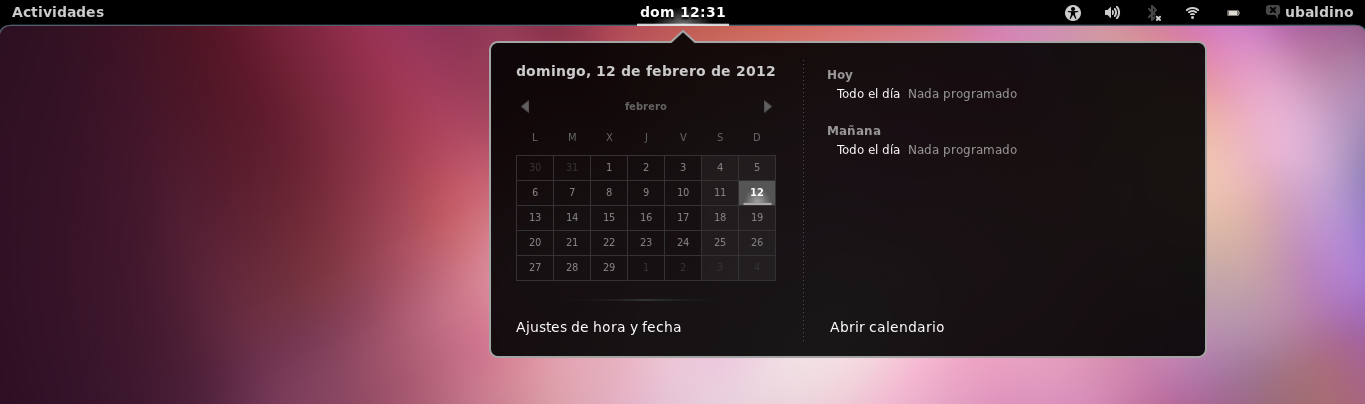
\includegraphics[scale=0.448]{gnome/barra.png}
\end{center}
Gnome es uno de los tantos escritorios que existen para las distribuciones basadas en linux.
En este caso UBUNTU 11.10 utiliza el escritorio o interfaz gráfica Gnome 3, y como es de esperar de un escritorio, los componentes principales del escritorio Gnome son:
\begin{itemize}
\item[-] Iconos que enlazan a archivos, carpetas o programas (accesos directos).
\item[-] Gnome Shell que es la barra de tareas y lanzador de aplicaciones. y tiene un gestor de ventanas con soporte OpenGL.
\begin{description}
\item[Gnome Shell] tiene un panel único en la parte superior, que contiene:
\begin{itemize}
 \item menú de usuario. 
 \item un botón “actividades”. 
 \item aplicaciones en ejecución.
 \item reloj.
 \item área de accesibilidad.
 \item control de volumen.
 \item información de la red.
 \item estado de la batería en el caso de un portátil.
\end{itemize}
En el arranque del sistema aparece dicho panel y el fondo de escritorio.
\end{description}
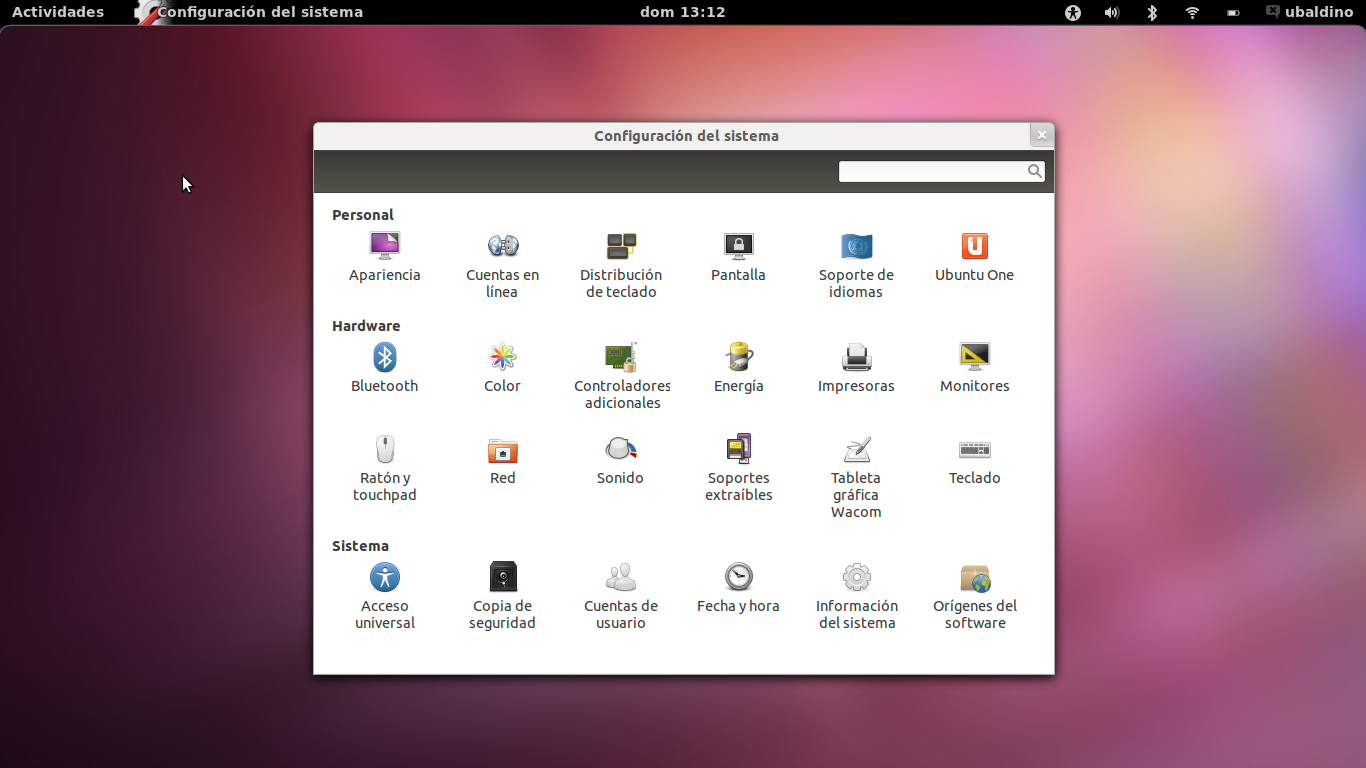
\includegraphics[scale=0.35]{gnome/Pantallazo3.png}\\ 
Al pulsar sobre “actividades” o acercar el ratón con rapidez a la esquina superior izquierda, se despliegan varios elementos nuevos:
\begin{itemize}
\item A la izquierda, un panel lanzador de aplicaciones,
\item Bajo el panel superior, un menú de dos opciones, “ventanas” y “aplicaciones”.
\item A la derecha, otro panel con una vista previa de las ventanas activas que actúa como selector de escritorios y por encima de éste, una caja de búsqueda.
\end{itemize}
Si tienes ya algún programa en ejecución, que por defecto se lanza a pantalla completa, la ventana o ventanas activas que su reducen su tamaño mostrando una leyenda informativa en la parte inferior de cada ventana. Cada acción que comporte cambios de tamaño o posición, vendrá acompañada de una elegante animación y otros efectos visuales.\\
El botón gráfico windows (ventanas), restaura la vista previa de aquellas que estén activas si las has perdido de vista por ejecutar cualquier otra acción.\\
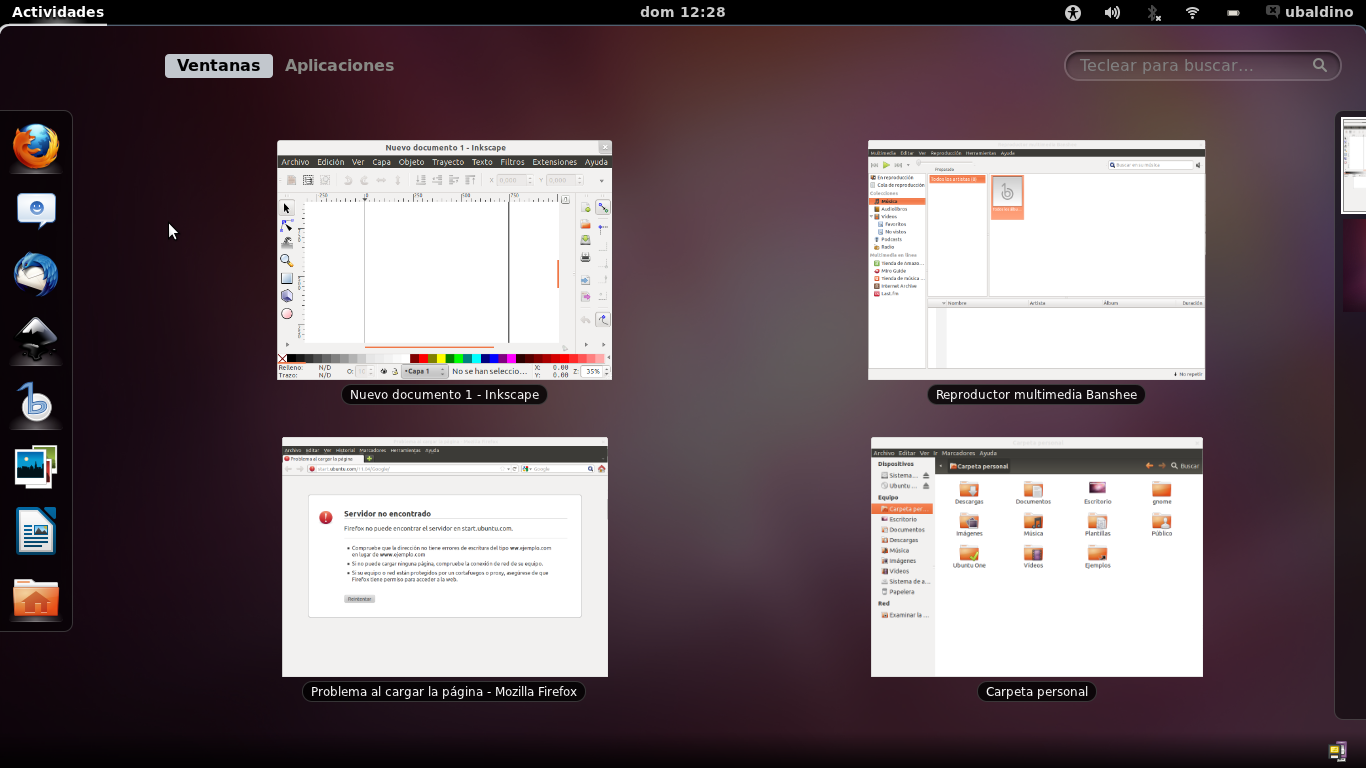
\includegraphics[scale=0.35]{gnome/Pantallazo4.png}\\ 

El botón aplications (aplicaciones), da paso a la representación mediante iconos de los programas instalados en la máquina.\\

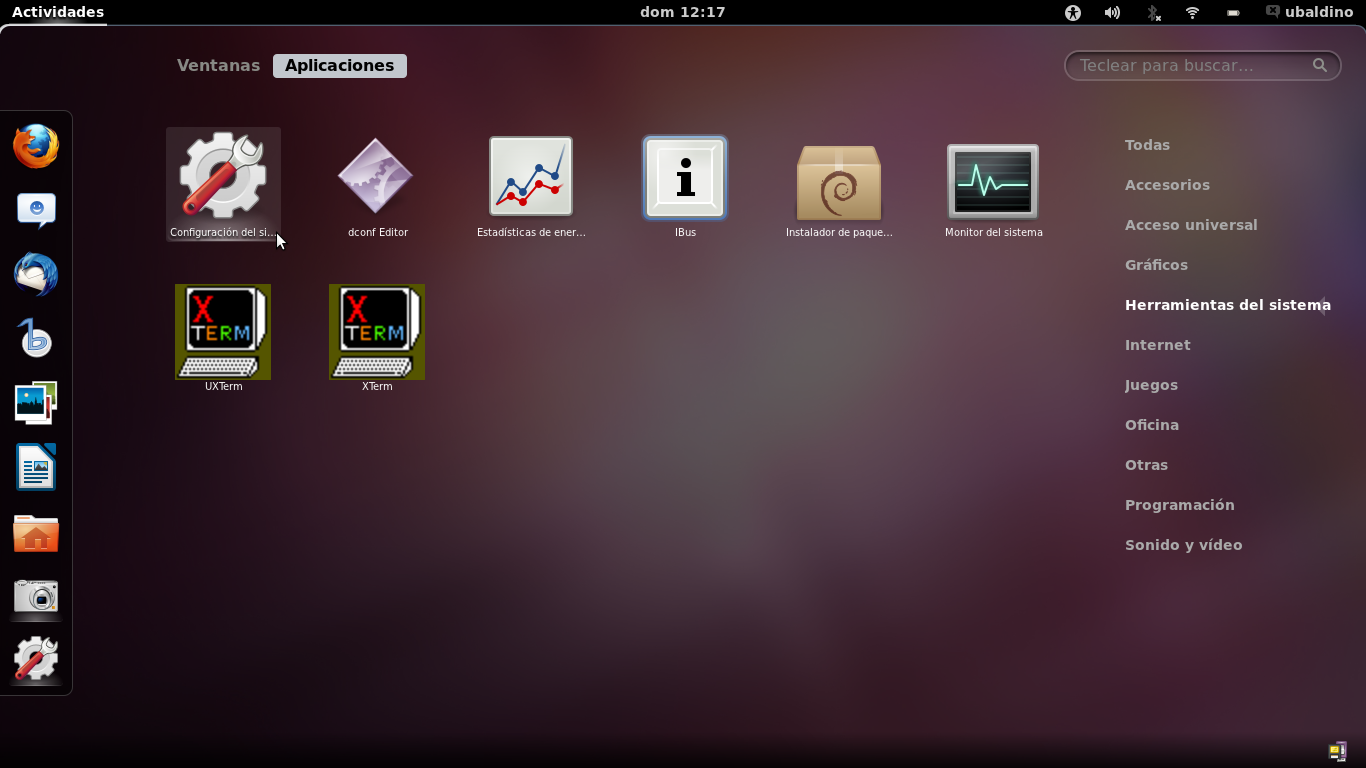
\includegraphics[scale=0.35]{gnome/Pantallazo5.png} \\
\underline{\bf Nota:} Note que cuando estamos en la presentación de los programas instalados en la maquina. El panel de la derecha porta un sistema de filtrado, clasificando los programas según las funcionalidades.\\

La caja de búsqueda es lo novedoso de gnome 3. Escribiendo las primeras letras de una aplicación, aparecerá de forma inmediata el icono correspondiente al programa y puedes lanzar la aplicación desde ahí. Y en la parte inferior de la pantalla muestra dos botones gráficos, que permiten extender la búsqueda en Wikipedia y Google.\\ 

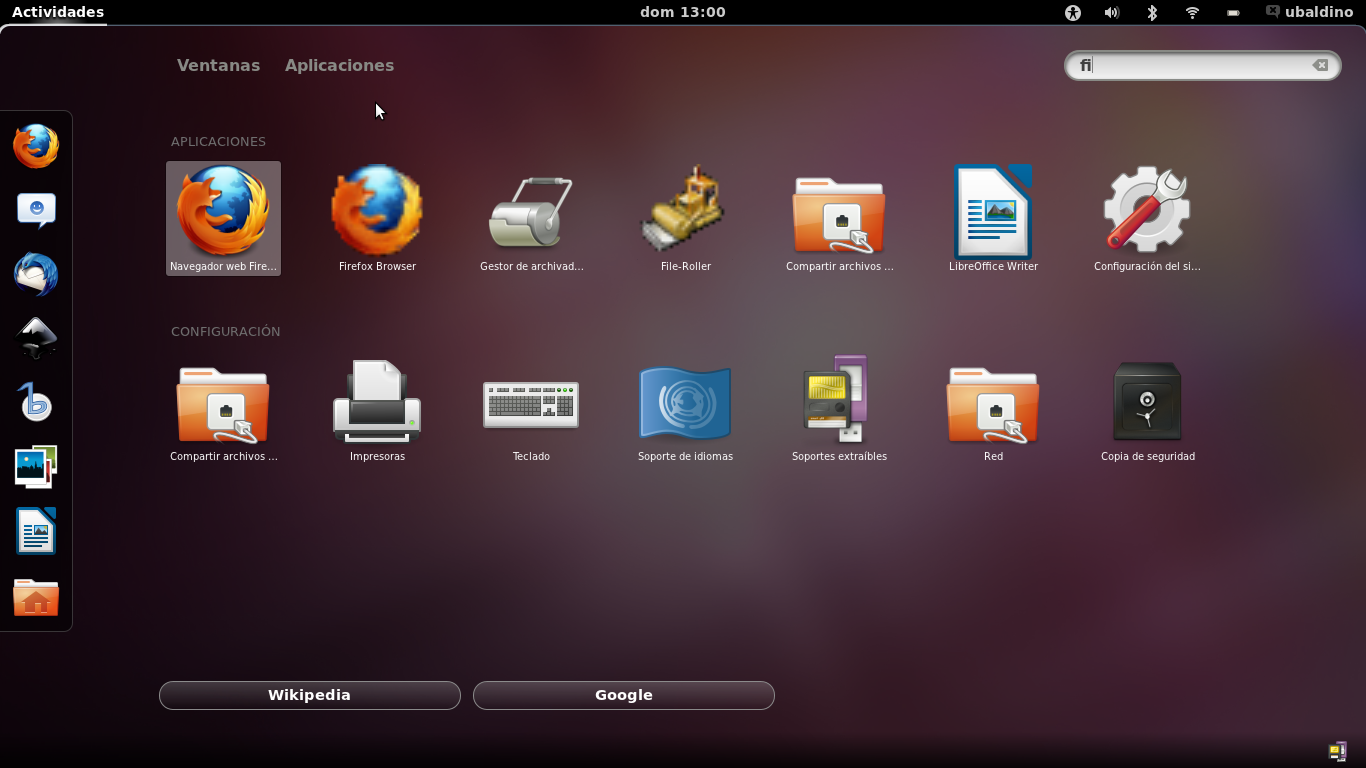
\includegraphics[scale=0.35]{gnome/Pantallazo6.png}\\ 

Por último, terminando nuestro recorrido en Gnome Shell, en la parte inferior derecha de la pantalla veremos el área de notificaciones y bandeja de mensajes, desde donde puedes contestar con el programa de mensajería instantánea.\\
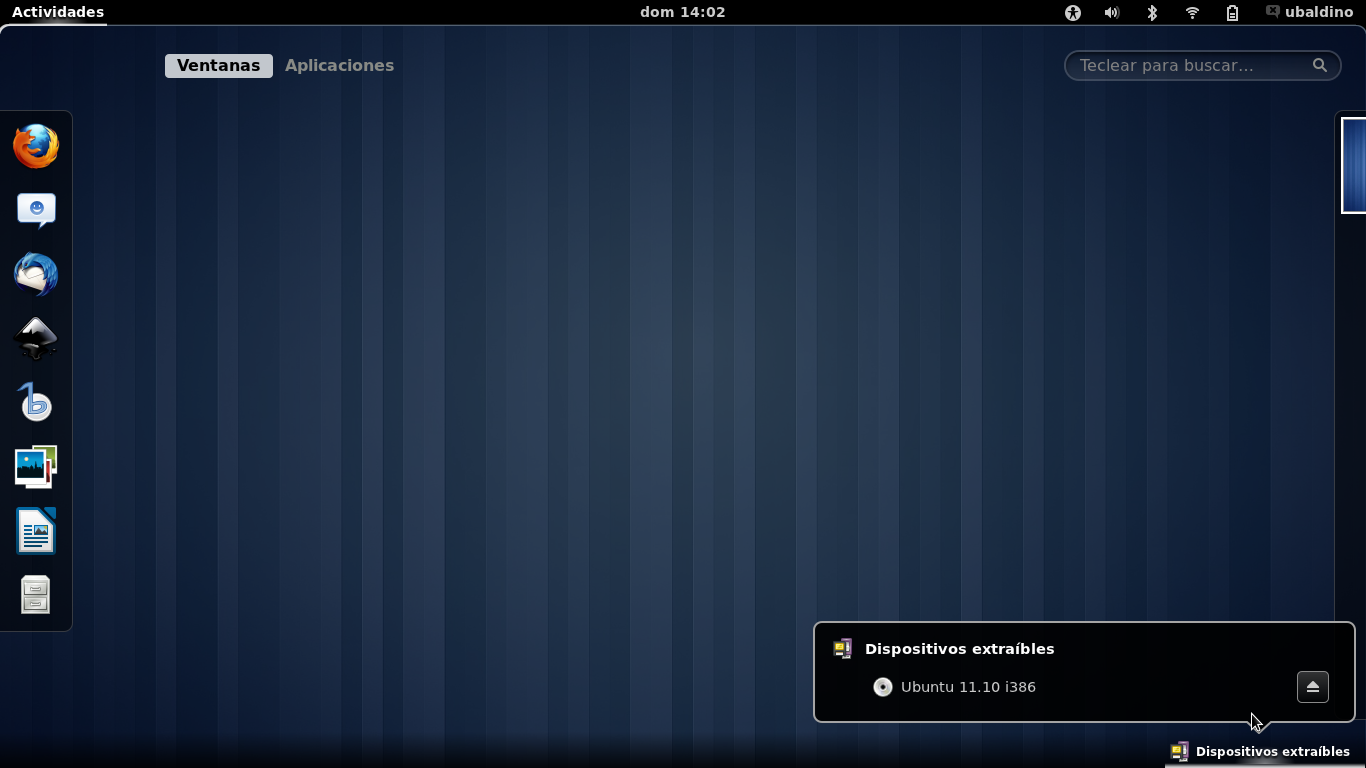
\includegraphics[scale=0.35]{gnome/Pantallazo7.png} 
\end{itemize}
\section{Ventanas y áreas de trabajo}
Como otros escritorios, GNOME usa ventanas para mostrar las aplicaciones en ejecución. Usando la vista y el tablero, puede lanzar aplicaciones nuevas y controlar qué ventana está activa.\\

Además de en las ventanas, también puede agrupar sus aplicaciones en áreas de trabajo. Visite los temas de ayuda de ventana y área de trabajo que se muestran a continuación para aprender mejor cómo usar estas características.

\subsection{Trabajar con ventanas}
\subsubsection{Cambiar entre ventanas}
Incluir todas las aplicaciones en el selector de ventanas hace que el cambio entre tareas sea un proceso sencillo y proporciona una imagen completa de las aplicaciones que están en ejecución.\\

{\bf Desde un área de trabajo:}
\begin{itemize}
\item Pulse Alt+Tab para mostrar el selector de ventanas.
\item Suelte la tecla Alt para seleccionar la siguiente ventana (resaltada) en el selector.
\item Otra forma, aún manteniendo pulsada la tecla Alt, pulse Tab para cambiar entre la lista de ventanas abiertas, o pulse Mayús+Tab para cambiar hacia atrás.
\end{itemize}
Las ventanas en el selector de ventanas se agrupan por aplicaciones. Las vistas previas de las aplicaciones con múltiples ventanas se despliegan cuando las pulsa. Pulse Alt y pulse la tecla Tab para recorrer la lista.\\
En el selector de ventanas, las aplicaciones de diferentes áreas de trabajo se dividen con separadores verticales.

\begin{itemize}
\item También puede moverse entre los iconos de aplicaciones en el selector de ventanas con las teclas $→$ o $←$, o seleccionar una pulsándola con el ratón.\\
Las vistas previas de las aplicaciones con una sola ventana se pueden mostrar con la tecla $↓$.
\end{itemize}
{\bf Desde la vista de Actividades:}
\begin{itemize}
\item Pulse en una ventana para cambiar a ella y salir de la vista previa. Si tiene varias áreas de trabajo abiertas, puede pulsar en cada una de ellas para ver las ventanas abiertas en cada área de trabajo.
\end{itemize}
\subsubsection{Encontrar una ventana perdida}
Una ventana en un área de trabajo diferente, u oculta detrás de otra ventana es sencilla de encontrar usando la vista de actividades:
\begin{itemize}
\item Abra la vista de actividades y asegúrese de que la vista de Ventanas está seleccionada. Si la ventana que está buscando está en el área de trabajo, se mostrará aquí como una miniatura. Para mostrarla de nuevo, simplemente pulse la miniatura, o
\item Pulse en diferentes áreas de trabajo en el selector de áreas de trabajo en la derecha de la pantalla para tratar de encontrar la ventana, o
\item Pulse con el botón derecho en la aplicación en el tablero y se listarán las ventanas abiertas. Pulse en la ventana de la lista a la que quiere cambiar.
\end{itemize}

{\bf Usando el selector de ventanas:}
\begin{itemize}
\item Pulse Alt+Tab para mostrar el selector de ventanas. Mantenga pulsada la tecla Alt y pulse Tab para cambiar entre la lista de ventanas abiertas, o pulse Mayús+Tab para cambiar hacia atrás.
\item Si una aplicación tiene múltiples ventanas abiertas, pulse Alt y la tecla Tab para pasar por ellas.
\end{itemize}
\subsubsection{Maximizar y des-maximizar (restaurar) una ventana}
Para maximizar o restaurar una ventana:
\begin{itemize}
\item Doble pulsación en la barra de títulos de la ventana.
\end{itemize}
Alternativamente, para maximizar:
\begin{itemize}
\item Pulse en la barra de título de una aplicación y arrástrela a la parte superior de la pantalla. Cuando el puntero del ratón toque la parte superior de la pantalla, toda la pantalla se iluminará. Suelte el botón del ratón para maximizar la pantalla.
\end{itemize}
Para restaurar la ventana a su tamaño original:
\begin{itemize}
\item Pulse en la barra de título de la aplicación y arrástrela hacia abajo desde la barra superior. Una vez separada de la barra superior volverá a un estado des-maximizado.
\end{itemize}
Pulse Alt y arrastre con el ratón en cualquier lugar de la ventana. Esto el permitirá mover la ventana. Algunas personas pueden encontrar esto más sencillo que pulsar en la barra de título de una aplicación.\\
También puede usar su teclado para maximizar una ventana. Pulse Alt+Espacio para mostrar el menú de la ventana, y pulse x.
\subsubsection{Operaciones de ventanas}
Las ventanas pueden redimensionarse u ocultarse para ajustarse a un flujo de trabajo
\begin{itemize}
\item {\bf Minimizar, restaurar y cerrar}\\
Para minimizar una ventana u ocultar una ventana:
\begin{itemize}
\item Pulse Alt+Space para mostrar el menú de la ventana. Entonces pulse n. La ventana desaparece en la esquina superior izquierda.
\end{itemize}
Para restaurar la ventana:
\begin{itemize}
\item Pulse en ella o en la vista de actividades o recupérela desde el selector de ventanas pulsando Alt+Tab.
\end{itemize}
Para cerrar la ventana:
\begin{itemize}
\item Pulse en la x en la esquina superior derecha de la ventana, o
\item Pulse Alt+F4, o
\item Pulse Alt+Espacio para mostrar el menú de la ventana. Entonces pulse la tecla c.
\end{itemize}
\item {\bf Redimensionar}\\
Si una ventana está maximizada no se puede redimensionar.\\

Para redimensionar su ventana horizontal y/o verticalmente:
\begin{itemize}
\item Mueva el puntero del ratón a cualquier esquina de la ventana hasta que se convierta en un \underline{puntero de esquina}. Pulse, mantenga y arrastre para cambiar el tamaño de la ventana en cualquier dirección.
\end{itemize}
Para redimensionar sólo horizontalmente:
\begin{itemize}
\item Mueva el puntero del ratón a cualquier lado de la ventana hasta que se convierta en un \underline{puntero lateral}. Pulse $+$ mantenga $+$ arrastre para cambiar el tamaño de la ventana en la dirección horizontal.
\end{itemize}
Para redimensionar sólo verticalmente:
\begin{itemize}
\item Mueva el puntero del ratón a la parte superior o inferior de la ventana hasta que se convierta en un \underline{puntero superior} o en un \underline{puntero inferior}, respectivamente. Pulse, mantenga y arrastre para cambiar el tamaño de la ventana en la dirección vertical.
\end{itemize}
\item {\bf Organizar ventanas en su área de trabajo}\\
Puede situar dos ventanas juntas. Arrastre una ventana por su barra de título hacia la izquierda hasta que el cursor toque el lado izquierdo de la pantalla. La mitad izquierda de la pantalla se iluminará. Suelte el ratón y la ventana se redimensionara para ocupar exactamente la mitad de su pantalla. Haga lo mismo para la otra ventana, arrastrándola a la derecha y soltando.
\end{itemize}
\subsubsection{Ventanas en mosaico}
Su forma de trabajo puede necesitar dos ventanas lado a lado para comprar resultados. Para llenar la pantalla con dos ventanas orientadas verticalmente:
\begin{itemize}
\item Pulse en la barra de título de una aplicación y arrástrela a la parte superior de la pantalla. Cuando el puntero del ratón toque la parte superior de la pantalla, toda la pantalla se iluminará. Suelte el botón del ratón para maximizar la pantalla.
\item Arrastre otra ventana a la parte derecha: cuando la mitad derecha de la pantalla esté resaltada, suélte la ventana. Cada una de las dos ventanas llena la mitad de la pantalla.
\end{itemize}
Pulsar Alt + y pulsar en cualquier parte de una ventana le ayudará a mover la ventana. Algunas personas pueden encontrar esto más sencillo que pulsar en la barra de título de una aplicación.
\subsection{Trabajar con áreas de trabajo}
\subsubsection{¿Que es un área de trabajo y cómo me ayudará?}
Las áreas de trabajo se refieren a la agrupación de ventanas en su escritorio. Puede crear muchas áreas de trabajo, las cuales actúan como escritorios virtuales. Las áreas de trabajo están destinadas a reducir el desorden y hacer que el escritorio sea sencillo de examinar.\\

Podría utilizar las áreas de trabajo para organizar su trabajo. Por ejemplo, podría tener todas sus ventanas de comunicación, tales como el correo electrónico y su programa de chat en un área de trabajo y el trabajo que está haciendo en un área de trabajo diferente. Su gestor de música podría estar en una tercera área de trabajo.\\

{\bf Usando áreas de trabajo:}
\begin{itemize}
\item En la vista de Actividades, mueva su cursor a la parte más a la derecha de la pantalla. Aparecerá un panel vertical con las áreas de trabajo en uso y con área de trabajo adicional vacía. Esto es el selector de áreas de trabajo.
\item Para añadir un área de trabajo, mueva una ventana de un área de trabajo existente hasta el área de trabajo vacía en el selector de áreas de trabajo. Esta área de trabajo contiene ahora la ventana que se dejó en ella, y debe aparecer un área de trabajo nueva vacía en la parte inferior.
\item Para quitar un área de trabajo, simplemente cierre todas las ventanas que tenga, o muévalas a otras áreas de trabajo.
\end{itemize}
Siempre hay al menos un área de trabajo.
\subsubsection{Cambie entre las áreas de trabajo}
\begin{itemize}
\item {\bf Usando el ratón:}\\
En la vista Actividades, pulse en un área de trabajo en el selector de áreas de trabajo en el lado derecho de la pantalla para ver las ventanas abiertas en ese área de trabajo. Pulse en cualquier miniatura de ventana para activar el área de trabajo.\\

\item {\bf Usando el teclado:}
\begin{itemize}
\item Pulse Ctrl+Alt+$↑$ para moverse a un área de trabajo que esté encima de la actual en el selector de áreas de trabajo.
\item Pulse Ctrl+Alt+$↓$ para mover a un área de trabajo que está debajo del área de trabajo actual en el selector de áreas de trabajo.
\end{itemize}
\end{itemize}
\subsubsection{Mover una ventana a un área de trabajo diferente}
\begin{itemize}
\item {\bf Usando el ratón:}
\begin{enumerate}
\item Abra la vista de Actividades y asegúrese de que está en la vista de Ventanas.
\item Pulse y arrastre la ventana a la derecha de la pantalla.
\item El selector de áreas de trabajo aparecerá.
\item Arrastre la ventana a un área de trabajo vacía. Este área de trabajo ahora contiene la ventana que se arrastró en ella y se creará una nueva área de trabajo vacía al final del selector de áreas de trabajo.
\end{enumerate}
\item {\bf Usando el teclado:}
\begin{enumerate}
\item Pulse sobre la ventana para hacerla activa.
\item Pulse Ctrl+Alt+Mayús+$↑$ para mover la ventana al área de trabajo encima del actual en el selector de áreas de trabajo.
\item Pulse Ctrl+Alt+Mayús+$↓$ para mover la ventana al área de trabajo debajo del actual en el selector de áreas de trabajo.
\end{enumerate}
\end{itemize}
\chapter{barra de menú}
\chapter{Personalización}
Se puede cambiar el aspecto y el comportamiento del escritorio Gnome para que se adapte a preferencias y necesidades personales. Algunos de los ajustes que puede querer cambiar incluyen:
\begin{itemize}
\item Configuración del teclado y el ratón.
\item Modificación de preferencias del teclado.
\item Configuración del ratón.
\item Fondo del escritorio.
\item Protector de pantalla.
\item Contraseña.
\item Sonidos.
\end{itemize}
Estos ajustes, entre otros, se pueden cambiar en el Centro de control.
\section{Herramientas del sistema}
Para acceder al centro de control, haga clic en {\bf actividades $=>$ aplicaciones $=>$ panel derecho herramientas del sistema $=>$ Configuración del sistema}. Este se encuentra dividido en las tres categorías siguientes:
\begin{description}
\item[Personal] Acceda aquí para cambiar los valores de configuración del fondo de escritorio. Puede modificar los temas, agregar o quitar idiomas y poder configurar la distribución del teclado que desee utilizar.
\item[Hardware] Permite configurar componentes de hardware, como tarjetas gráficas, monitores, impresoras o para configurar los accesos directos y los atajos de teclado, así como instalar dispositivos de red y configurar la conexión de red.
\item[Sistema] Permite configurar valores del sistema como la fecha y la hora y cambiar
la contraseña de entrada o los valores de accesibilidad.
También podrá cambiar direcciones de los servidores de software y obtener información de su sistema 
\end{description}
\begin{center}
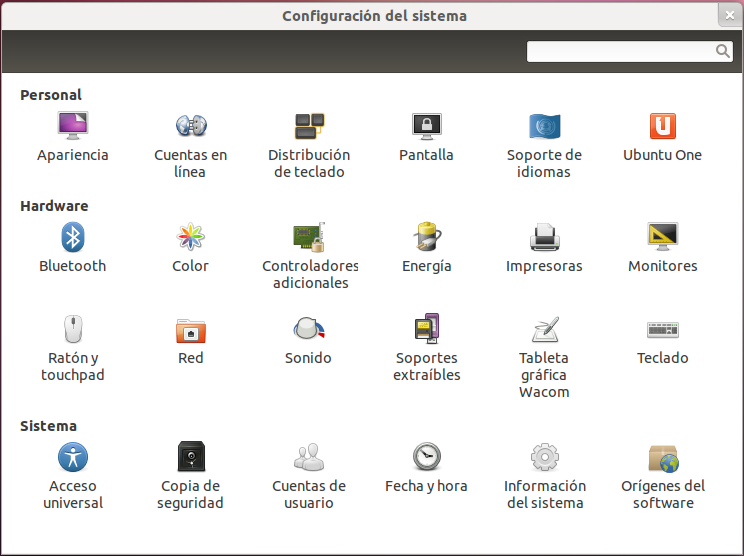
\includegraphics[scale=0.6]{gnome/Pantallazo31.png}
\end{center}
Para cambiar algunos de los valores globales del sistema, Gnome solicitará
la contraseña del usuario Administrador. Es el caso principalmente de los
valores del administrador, que incluyen la mayor parte de los valores de configuración
del hardware, la interfaz gráfica del usuario, el acceso a Internet, la seguridad, la
administración de usuarios o la instalación de software, así como las actualizaciones y
la información del sistema.
\section{Personal}
En esta sección veremos ejemplos sobre cómo configurar algunos aspectos personales del escritorio Gnome, como la accesibilidad y la configuracion de la hora y fecha o la compatibilidad con la tecnología de asistencia, así como sobre la forma de cambiar la contraseña o gestionar anillos de claves virtuales.
	\subsection{Apariencia}
	\begin{center}
	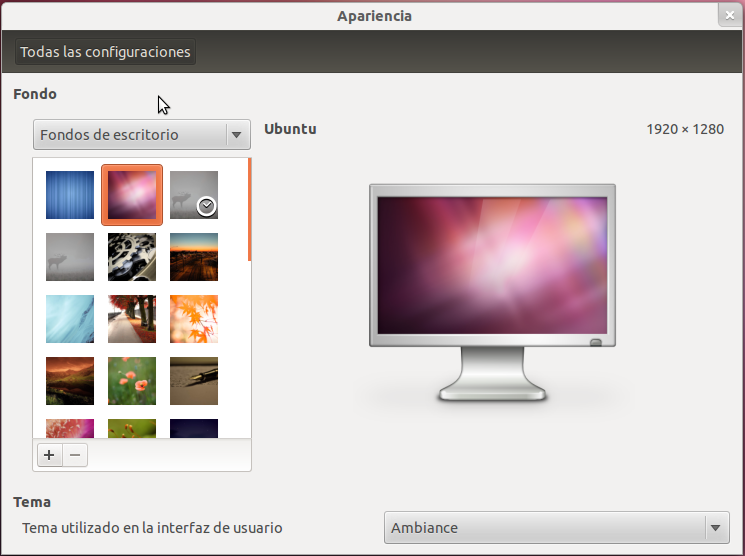
\includegraphics[scale=0.6]{gnome/apariencia.png}
	\end{center}	
		\begin{itemize}
			\item {\large \bf Cambiar el fondo del escritorio}
				
					Puede cambiar la imagen usada en el fondo del escritorio o establecer un color simple o degradado.\\

Seleccione una imagen o un color. La configuración se aplicará inmediatamente.\\

Existen tres opciones en la lista desplegable en la izquierda.
\begin{itemize}
\item Seleccione Fondos de escritorio para usar una de las muchas imágenes de fondo profesionales con las que se distribuye GNOME. Algunos fondos de escritorio son parcialmente transparentes y permiten mostrar un color de fondo a través de ellos. Para esos fondos de escritorio, existirá un botón de selección de color en la esquina inferior derecha.
\item Seleccione la carpeta Imágenes para usar una de sus propias fotografías de su carpeta Imágenes. La mayoría de los gestores de fotos almacenan las fotos aquí.
\item Seleccione Color y gradientes para ajustar un color plano o un gradiente lineal. Los botones selectores de color aparecerán en la esquina inferior derecha.
\end{itemize}
También puede buscar una imagen en su equipo pulsando el botón +. Cualquier imagen que añada de esta manera se mostrará en la carpeta de Imágenes.\\
Puede quitarla de la lista seleccionándola y pulsando el botón -. Quitar una imagen de la lista no eliminará el archivo original.

			\item {\large \bf Cambiar el tema del escritorio}
			Un tema es un grupo de ajustes que especifican el aspecto visual de una parte del escritorio. Los usuarios pueden seleccionar temas para cambiar el aspecto del escritorio.\\

Seleccione una tema de su preferencia. La configuración se aplicará inmediatamente.\\
Un tema contiene ajustes que afectan a distintas partes del escritorio, como se describe
a continuación:
\begin{description}
\item[Controles] El ajuste de controles de los temas determina el aspecto visual de las ventanas, paneles y applets. También determina el aspecto visual de los elementos de la interfaz compatible con GNOME que se muestran en las ventanas, paneles y applets (como menús, iconos y botones). Algunas de las opciones de ajuste de los controles disponibles están diseñadas para necesidades de accesibilidad especiales.
\item[Marco de las ventanas] El ajuste de los marcos de las ventanas de un tema determina únicamente el aspecto de los marcos que rodean las ventanas.
\item[Icono] El ajuste de los iconos de un tema determina el aspecto de los iconos en los paneles y el fondo del escritorio.
\end{description}
		\end{itemize}
	\subsection{Distribución del teclado}
	Los teclados vienen en cientos de distribuciones diferentes para distintos idiomas. Incluso para un solo idioma pueden existir muchas distribuciones de teclado, como la distribución Dvorak para el inglés. Puede hacer que su teclado se comporte como un teclado con una distribución diferente, independientemente de que letras y símbolos tenga escritos en las teclas. Esto es útil si tiene que usar varios idiomas a menudo.\\

Abra distribución del teclado\\

Nos encontraremos con cuatro pestañas que veremos a continuación:
\begin{itemize}
	\item {\large \bf Idioma}\\
	En esta pestaña puede anadir varios idiomas para que el teclado se comunique con nuestro sistema\\
    Pulsando el botón +, añade un idioma\\
    Pulsando el boton -, elimina un idioma
\begin{center}
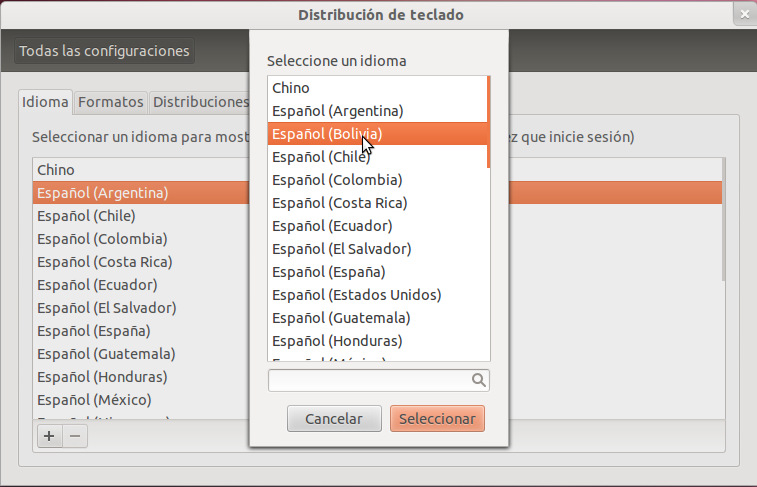
\includegraphics[scale=0.6]{gnome/idioma1.png} 
\end{center}
	\item {\large \bf Formatos}\\
		Esta pestaña te mostrara la forma de mostrar información que sera adecuada a tu zona para la cual elegimos.
\begin{center}
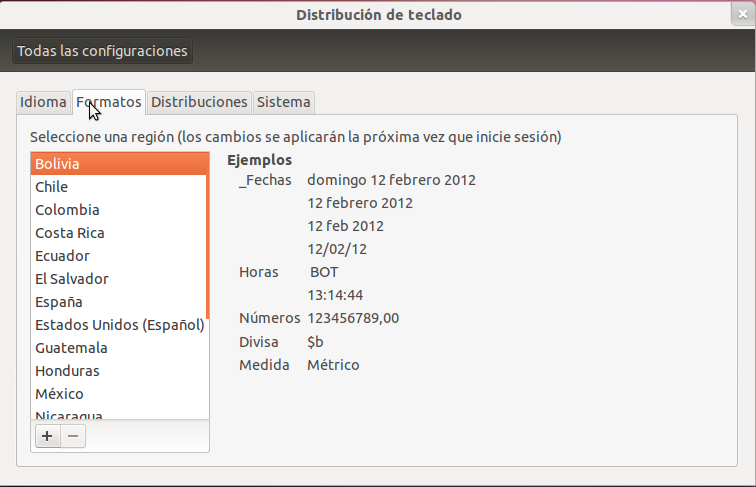
\includegraphics[scale=0.6]{gnome/formato.png} 
\end{center}
Podemos añadir como también eliminar regiones.\\ 
		Cuando cambia su región para los formatos, sólo lo cambia para su cuenta después de iniciar la sesión.
	\item {\large \bf Distribuciones}\\
	Los teclados vienen en cientos de distribuciones diferentes para distintos idiomas. Incluso para un solo idioma pueden existir muchas distribuciones de teclado, como la distribución Dvorak para el inglés. Puede hacer que su teclado se comporte como un teclado con una distribución diferente, independientemente de que letras y símbolos tenga escritos en las teclas. Esto es útil si tiene que usar varios idiomas a menudo.
Pulse en su nombre en la barra superior y seleccione Configuración del sistema.\\

Seleccione la pestaña Distribuciones.\\
Pulse el botón +, seleccione una distribución y pulse Añadir. Puede añadir hasta cuatro distribuciones.\\
Puede tener una vista previa de una imagen o cualquier distribución seleccionando en la lista y pulsando la imagen de teclado, o pulsando Vista previa en la ventana emergente cuando añade una distribución.\\
Cuando se añaden varias distribuciones, puede cambiar entre ellas utilizando el icono de distribución de teclado en la barra superior. La barra superior mostrará una cadena corta de identificación de la distribución actual, tal como es para la distribución estándar de español. Pulse en el indicador de la distribución y seleccione la que quiera usar en el menú.\\
Cuando se usan varias distribuciones, se puede elegir entre tener todas las ventanas con la misma distribución o asignar una distribución diferente a cada ventana. Este último resulta interesante, por ejemplo, si esta escribiendo un articulo en otro idioma en una ventana del procesador de textos. Cada ventana recordara su selección de teclado conforme vaya pasando de una ventana a otra.\\

De manera predeterminada, las nuevas ventanas usaran la distribución de teclado predeterminada. En su lugar, puede elegir que usen la distribución de la ventana que estuviera usando antes. La distribución predeterminada es la situada al principio de la lista. Use los botones $\uparrow$ y $\downarrow$ para subir o bajar las distribuciones dentro de la lista.
	\item {\large \bf Sistema}\\
	Simplemente muestra los ajustes del sistema.	
	\begin{center}
		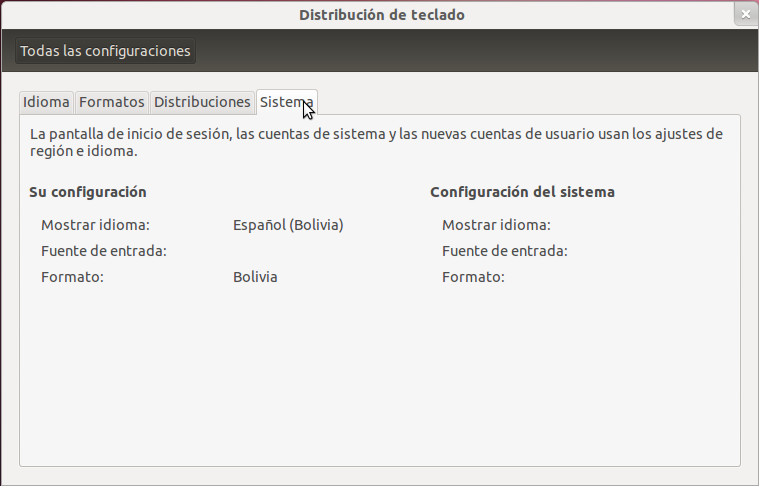
\includegraphics[scale=0.6]{gnome/sistema1.png} 
    \end{center}
\end{itemize}
\subsection{Pantalla}
Puede cambiar el brillo de su pantalla para ahorrar energía o hacerla más legible en condiciones de mucha luz ambiental. También puede hacer que la pantalla se atenúe automáticamente cuando se consume batería o apagarla automáticamente cuando no se use la pantalla.\\

Establecer el brillo\\

Abra Pantalla.
Mueva el deslizador de Brillo para obtener un valor confortable.\\

Muchas portátiles tienen teclados con teclas especiales para ajustar el brillo. Éstas tienen una imagen que parece un sol y están ubicadas en las teclas de función en la parte superior. Mantenga pulsada la tecla Fn para usar estas teclas.\\

Seleccione oscurecer para ahorrar energía, la pantalla se reducirá  automáticamente cuando esté usando la batería.\\
La luz de fondo de su pantalla puede consumir mucha energía y reducir significativamente el tiempo que durará la batería hasta que tenga que volver a cargarla.\\
La pantalla se apagará automáticamente cuando lleve un tiempo sin usarla.\\
Esto solo afecta a la pantalla, y no apaga su equipo. Puede ajustar el tiempo que tiene que estar inactivo en la lista desplegable Apagar después de:
\begin{center}
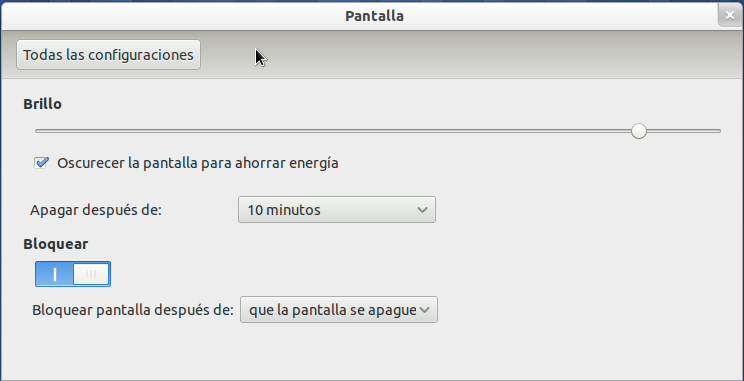
\includegraphics[scale=0.6]{gnome/pantallaa1.png} 
\end{center}
\subsection{Soporte de idiomas}
En esta sección aparecen los idiomas de soporte para las ventanas en orden por países por defecto esta primero España, pero puedes cambiar al país de tu preferencia con tan solo arrastrándolo hasta la posición que prefieras.
\begin{center}
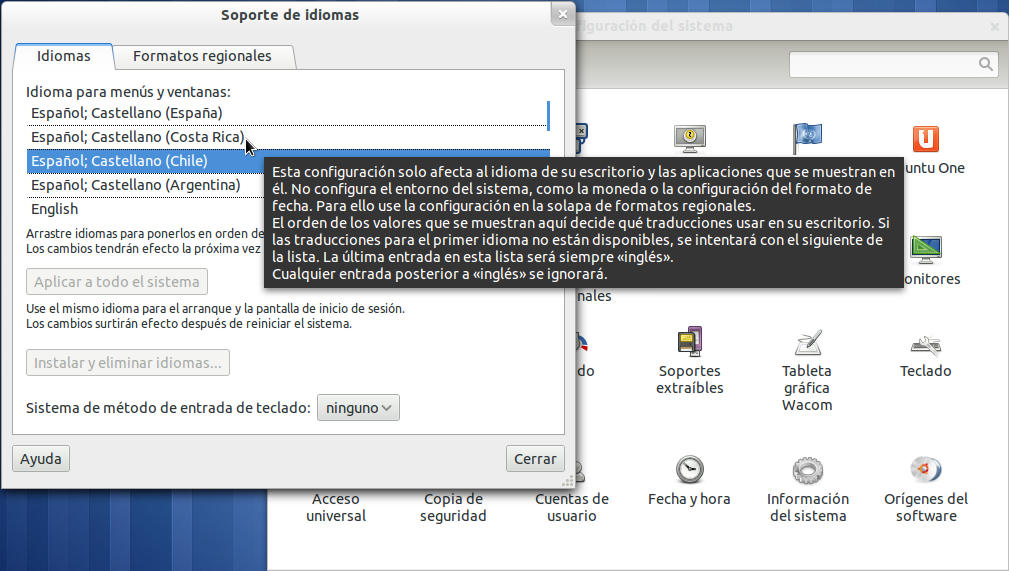
\includegraphics[scale=0.6]{gnome/idiomas2.png} 
\end{center}
En formatos regionales simplemente eliges el idioma y conjuntamente a la región de tu preferencia.
\begin{center}
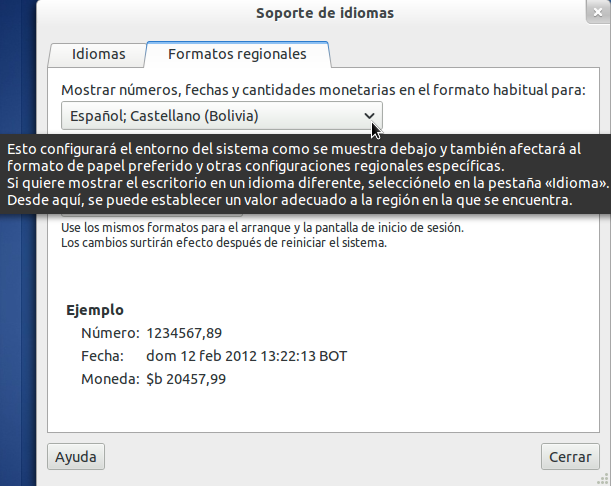
\includegraphics[scale=0.6]{gnome/idiomas3.png} 
\end{center}
%---------------------
\section{Hardware}
En esta sección veremos las configuraciones del hardware del escritorio Gnome, como las preferencias del teclado y del ratón, la gestión de unidades y medios extraíbles o la resolución de la pantalla.
\subsection{Modificación de preferencias del teclado}
Para modificar algunos valores de configuración, como las preferencias de repetición
automática o las sesiones de descanso de escritura, haga clic en Ordenador $>$ Centro
de control $>$ Hardware $>$ Teclado
\begin{enumerate}
\item En la ficha Teclado, puede definir algunas preferencias del teclado de carácter general, como habilitar la repetición con opciones de retardo y velocidad individuales, o habilitar e inhabilitar el parpadeo del cursor y definir la velocidad. Para obtener más información sobre cada una de las opciones, haga clic en Ayuda.
\item Para seleccionar el modelo del teclado, haga clic en la pestaña Distribuciones, haga clic en el botón Examinar y seleccione el modelo de la lista.
\item Para añadir una nueva distribución de idioma, haga clic en Añadir y elija una distribución de la lista. Puede seleccionar distintas distribuciones para ajustarlas a configuraciones regionales diferentes. Defina una distribución con el valor Por defecto.
\item En la pestaña Descanso de escritura puede definir las preferencias correspondientes. Para obtener más información sobre cada una de las opciones, haga clic
en Ayuda.
\item Cuando haya definido todas las opciones según sus preferencias, haga clic en Cerrar.
\end{enumerate}
\subsection{Monitores}
Puede cambiar los detalle del monitor como:
\begin{itemize}
\item La proporción entre la altura y la anchura (resolución).
\item Si su monitor puede girar físicamente en muchas direcciones. Puede cambiar la rotación de la pantalla. Puede elegir la rotación que quiere para su pantalla en la lista desplegable Rotación. 
\end{itemize}
\begin{center}
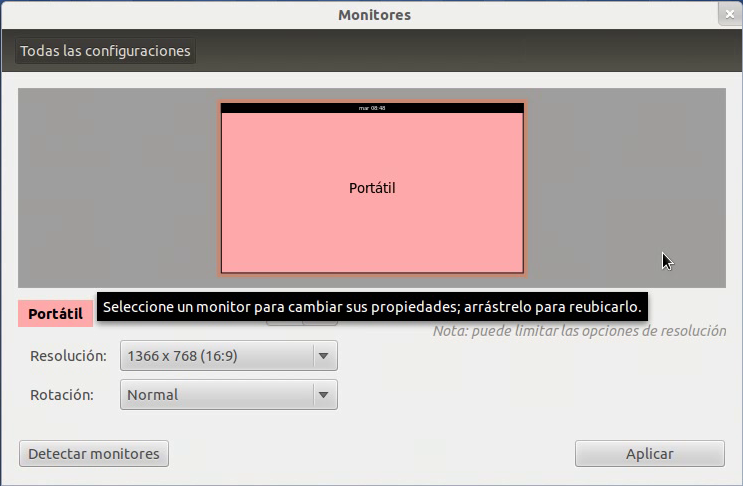
\includegraphics[scale=0.6]{gnome/monitor.png} 
\end{center}

\subsection{Ratón y Touchpad}
Entrando en la parte de Ratón y touchpad. \\
Seleccionando la pestaña Ratón, veras las siguientes opciones.
\begin{itemize}
\item{\large \bf Ratón}\\
\begin{center}
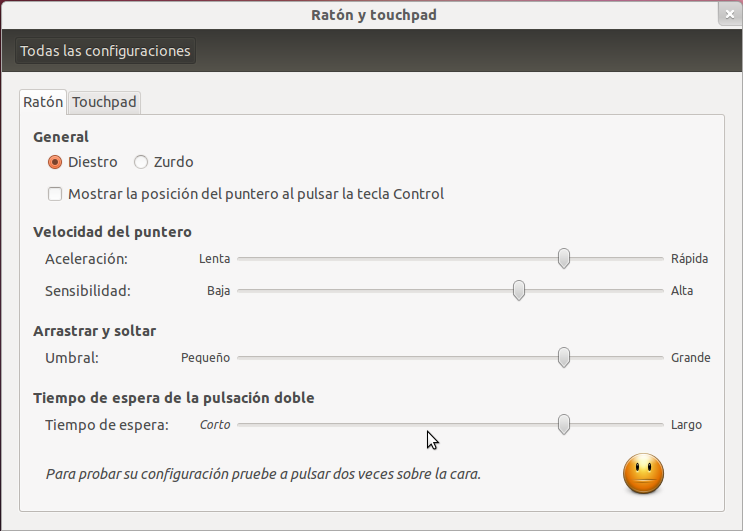
\includegraphics[scale=0.6]{gnome/raton.png} 
\end{center}
\begin{itemize}
\item{\bf General}\\
Puede intercambiar el comportamiento de los botones izquierdo y derecho de su ratón o touchpad para poder estar más cómodo.\\
Seleccione Zurdo.
Este ajuste afectará tanto a su ratón como a su touchpad, así como a cualquier otro dispositivo apuntador.\\

Al activar la opción de mostrar la posición del puntero al pulsar la tecla control.\\
Pulsando Ctrl se visualizará una animación que aparecerá brevemente en la posición del puntero.
\item{\bf Velocidad del puntero}\\
Si el puntero se mueve demasiado deprisa o despacio cuando mueve el ratón, puede ajustar la sensibilidad del puntero y la aceleración para estos dispositivos.\\

Ajuste los deslizadores de Aceleración y Sensibilidad hasta que el movimiento del puntero le sea cómodo.
\item{\bf Arrastrar y soltar}\\
Cuando se pulsa sobre algo, no es raro que su mano se mueva un poco durante el tiempo que pasa entre que pulsa el botón y lo suelta. Por esa razón, el proceso de arrastrar solo empieza si se mueve el puntero pasado un cierto umbral, para que no empiece a arrastrar accidentalmente cada vez que pulse sobre algo.\\

En Arrastrar y soltar, ajuste el deslizador del Umbral a un valor que le resulte cómodo. Pruebe a mover la ventana de opciones arrastrando la barra de título para probar el valor actual.\\

Este ajuste afectará tanto a su ratón como a su touchpad, así como a cualquier otro dispositivo apuntador.
\item{\bf Tiempo de espera de la pulsación doble}\\
La doble pulsación solo sucede cuando pulsa el botón del ratón dos veces lo bastante rápido. Si se tarda mucho en pulsar la segunda vez, obtendrá dos pulsaciones separadas, no una doble pulsación. Si tiene dificultados en pulsar el ratón tan deprisa debería incrementar el tiempo de espera.\\

En Tiempo de espera de la pulsación doble, ajuste el deslizador Tiempo de espera a un valor que considere confortable. Use la cara sonriente junto al deslizador para probar su configuración. Una pulsación simple lo hará sonreír. Una pulsación doble lo hará sonreír de oreja a oreja.\\

Este ajuste afectará tanto a su ratón como a su touchpad, así como a cualquier otro dispositivo apuntador.
\end{itemize}

\item{\large \bf Touchpad}\\
Puedes pulsar, hacer dobles pulsaciones, arrastrar y desplazarse usando solo el touchpad, sin usar botones físicos aparte.\\
Solo estará disponible si su equipo tiene uno.
	\begin{center}
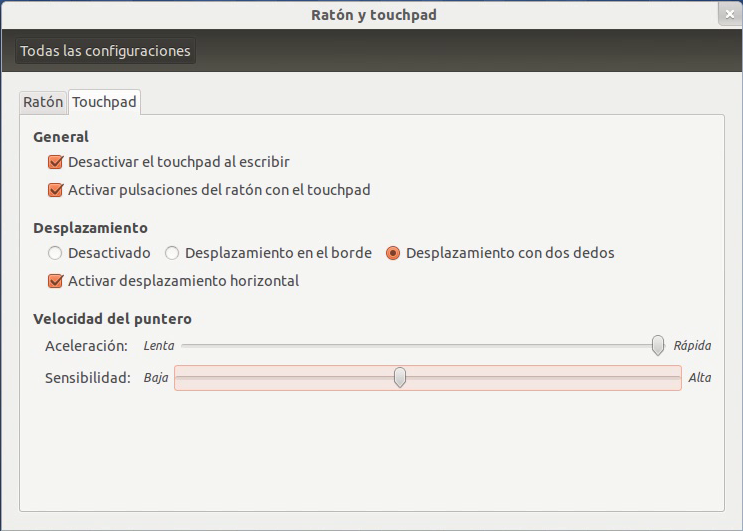
\includegraphics[scale=0.6]{gnome/touchpad.png}
\end{center} 
	\begin{itemize}
\item{\bf General}\\
Puedes activar o desactivar el touchpad cuando estas escribiendo o el acto de golpear y arrastrar con los dedos en el touchpad.\\ 

Para pulsar, pulsar dos veces y arrastrar con su touchpad seleccione Activar\\ pulsaciones del ratón con el touchpad.\\

Para pulsar toque el touchpad.\\
Para una doble pulsación, toque dos veces.\\
Para arrastrar un elemento, toque dos veces pero no levante su dedo después del segundo toque. Arrastre el elemento a donde quiera y después levante su dedo para soltarlo.\\
Si su touchpad es multitáctil, pulse con el botón derecho del ratón usando dos dedos a la vez. De lo contrario necesitará usar los botones del hardware para pulsar con el botón derecho del ratón. Para ver un método de pulsación derecha del ratón sin usar el segundo botón del ratón consulte la Simular una pulsación derecha del ratón.
\item{\bf Desplazamiento}\\
Si su touchpad soporta multi-toques puede elegir desplazamientos usando su touchpad, bien usando los bordes del touchpad o bien usando dos dedos.\\
\begin{itemize}
\item Seleccione Desplazamiento en el borde en Desplazamiento para hacer desplazamientos usando el borde de su touchpad.\\ Cuando está seleccionado, al arrastrar su dedo arriba y abajo por el lateral derecho de su touchpad se desplazará verticalmente.\\ Si además selecciona Activar desplazamiento horizontal, al arrastrar su dedo a izquierda y derecha por el borde inferior del touchpad se desplazará horizontalmente.

\item Seleccione Desplazamiento con dos dedos en Desplazamiento para desplazarse con dos dedos.\\
Cuando está seleccionado, el acto de golpear y arrastrar con un solo dedo funcionará como siempre, pero si arrastra dos dedos por cualquier zona del touchpad, hará un desplazamiento.\\ Si además selecciona Activar desplazamiento horizontal, podrá mover sus dedos a izquierda y derecha para desplazarse horizontalmente. Asegúrese de dejar un poco de espacio entre sus dedos. Si sus dedos están demasiado juntos, el touchpad podría creer que se trata de un único dedo grande.
\end{itemize}
\item{\bf Velocidad del puntero}\\
Si el puntero se mueve demasiado deprisa o despacio cuando usa el touchpad, puede ajustar la sensibilidad del puntero y la aceleración para este dispositivo.\\

Ajuste los deslizadores de Aceleración y Sensibilidad hasta que el movimiento del puntero le sea cómodo.\\

La sensibilidad es la velocidad inicial del puntero al mover su ratón.\\
Cuanto más mueva el ratón, más rápidamente se mueve el puntero con relación a su movimiento. Esto le ayuda a mover el puntero por la pantalla sin levantar la mano, mientras que le permite apuntar y pulsar de manera precisa. La aceleración controla este comportamiento.
\end{itemize}
\end{itemize}
\subsection{Red}
Entrando en la configuración de la red, encontraras dos opciones o tres si tienes adaptador de conexión inalámbrica.
\begin{itemize}
\item{\bf Cableada}
\begin{center}
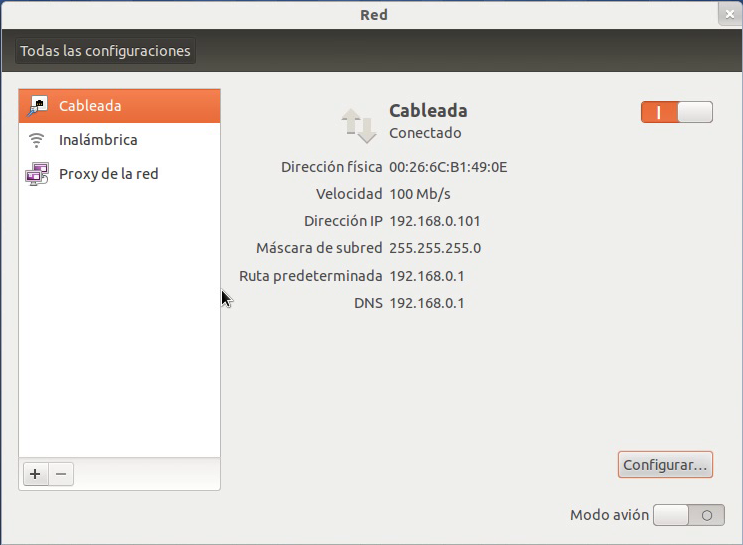
\includegraphics[scale=0.6]{gnome/cableada.png} 
\end{center}
Para configurar la mayoría de las conexiones a redes cableadas, todo lo que necesita es conectar un cable de red. El icono de red en la barra superior dará vueltas o parpadeará durante varios segundos y después cambiara al icono de un zócalo cuando esté conectado.\\
Si esto no ocurriera, deberá asegurarse primero de que su cable de red está conectado.\\

Puede habilitar o deshabilitar la conexión de red presionando el botón de activar/desativar.
\item{\bf Inalámbrica}
\begin{center}
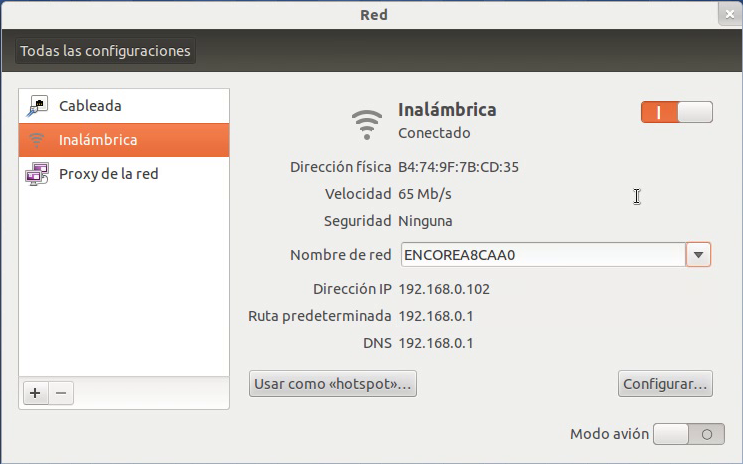
\includegraphics[scale=0.6]{gnome/inalambrica.png} 
\end{center}
Si tiene un equipo con una tarjeta inalámbrica que funcione puede conectarse a una red inalámbrica cercana para obtener acceso a Internet, ver archivos compartidos en la red y demás.\\

Puedes encender o apagar.\\
Activar el modo avión.\\
Configurar la red inalámbrica.\\

Para conectarse a una red pulse en el nombre de la red a la que quiere conectarse.\\
Si el nombre de la red no está en la lista, pruebe a pulsar Más para ver si la red está más abajo en la lista. Si sigue sin verla, puede que esté fuera del área de cobertura o puede que la red esté oculta.\\
Si la red está protegida por una contraseña (clave de cifrado), introduzca la contraseña cuando se le pida y pulse Conectar.\\
Si no conoce la clave, puede que esté escrita en la parte inferior del enrutador inalámbrico o de la estación base, en el manual de instrucciones, o puede tener que preguntar a la persona que administra la red inalámbrica.\\
El icono de red cambiará su apariencia según el equipo intente conectarse a la red.\\
Si la conexión se realiza correctamente, el icono cambiará a un punto con varias barras por encima. Más barras indican una conexión más fuerte a la red. Si no hay muchas barras, las conexión es débil y puede no ser posible.\\

Si la conexión no tiene éxito, se le puede preguntar su contraseña otra vez, o simplemente puede decirle que la conexión se ha desconectado. Hay varias razones que pueden hacer que esto pase; puede haber introducido mal la contraseña, la señal inalámbrica es muy débil o la tarjeta inalámbrica de su equipo tiene un problema, por ejemplo. Consulte el solucionador de problemas de red inalámbrica para obtener más ayuda.\\

Una conexión más fuerte a una red inalámbrica no significa necesariamente que vaya a tener una conexión a Internet más rápida, o que vaya a tener una velocidad de descarga mayor. La conexión inalámbrica conecta su equipo al dispositivo que proporciona la conexión a Internet (como un enrutador o un módem), pero las dos conexiones son diferentes, y por lo tanto tiene velocidades distintas.\\

{\large \bf hotspot}
\begin{center}
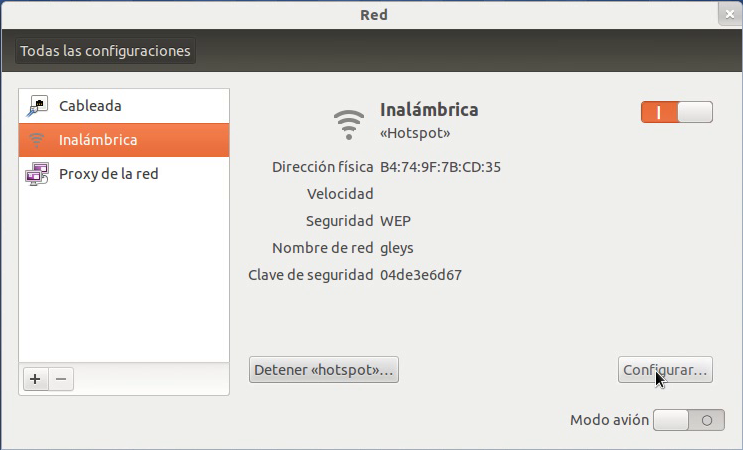
\includegraphics[scale=0.6]{gnome/hotspot.png} 
\end{center}
Puede usar su equipo como un hotspot inalámbrico. Esto permite a otros dispositivos conectarse a su equipo sin necesidad de una red aparte, y permite a su equipo compartir una conexión a Internet configurada en otra interfaz, como una red cableada o una red de banda ancha móvil.\\

Pulse el botón Usar como hotspot.\\
Si ya está conectado a una red inalámbrica, se le preguntará si quiere desconectarse de esa red.\\
Un adaptador inalámbrico sólo puede conectarse o crear una única red al mismo tiempo.\\
Pulse Crear hotspot para confirmar.\\

Se generan automáticamente un nombre de red (SSID) y una clave de seguridad. El nombre de red estará basado en el nombre de su equipo. Otros dispositivos necesitarán esta información para conectarse al hotspot que acaba de crear.\\

\begin{multicols}{2}
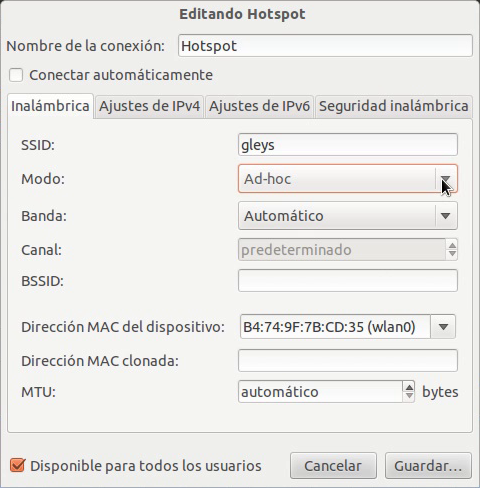
\includegraphics[scale=0.6]{gnome/hotspotC.png}

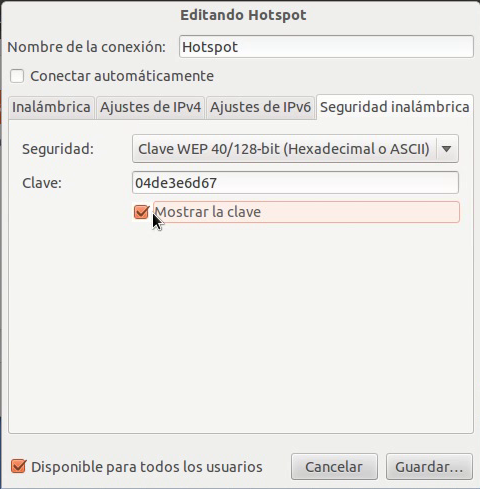
\includegraphics[scale=0.6]{gnome/hotspotS.png}
\end{multicols}
\end{itemize}

\subsection{Sonido}
Para cambiar el volumen del sonido, mueva el control deslizante de volumen a la derecha o a la izquierda. Puede desactivar completamente el sonido llevando el deslizador al extremo izquierdo.\\

Algunos teclados tienen teclas que le permiten controlar el volumen. Normalmente representan altavoces estilizados emitiendo ondas y frecuentemente están cerca de las teclas F en la parte superior. En los portátiles, normalmente están en las teclas F. Para usarlos mantenga pulsada la tecla Fn en su teclado.\\

Por supuesto, si tiene altavoces externos, también puede cambiar el volumen con el control de volumen en los propios altavoces. Algunos auriculares tienen también un control de volumen.

Ahora veremos un poco de las diferentes pestañas que hay en la opción de sonido.\\
\begin{itemize}
\item{\bf Efectos de sonido}\\
\begin{center}
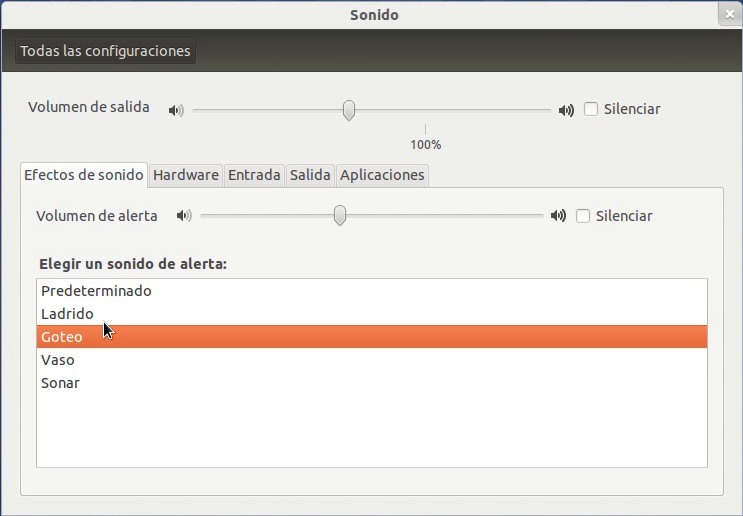
\includegraphics[scale=0.6]{gnome/efectos.png} 
\end{center}
Puede elegir diferentes sonidos para las alertas, establecer el volumen de alerta con independencia de su volumen de sistema, o desactivar los sonidos de alerta por completo.\\

En la pestaña Efectos de sonido, seleccione un sonido de alerta. Cada sonido se reproducirá cuando pulse en él, de manera que podrá oír como suena.\\

Use el deslizador de volumen en la pestaña Efectos de sonido para ajustar el volumen del sonido de alerta. Esto no afectará al volumen de la música, películas u otros archivos de sonido.\\
Para desactivar completamente los sonidos de alerta, seleccione Silenciar en la pestaña Efectos de sonido.\\
El equipo reproducirá un sonido de alerta simple para ciertos tipos de mensajes y eventos.
\item{\bf Hardware}\\
Si es que su maquina tuviera varias tarjetas de sonido incorporadas, usted podrá elegir la que va a utilizar.\\
Para percatarse de que dicho hardware funciona bien, pruebe altavoces presionando \underline{probar altavoces} 
\begin{center}
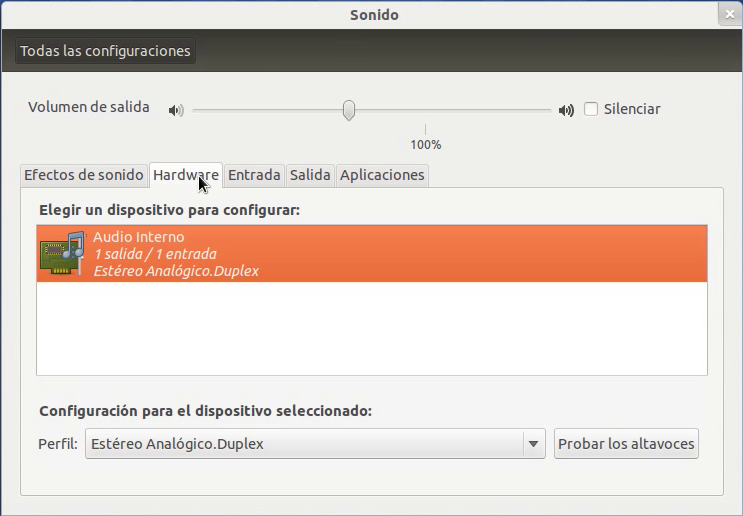
\includegraphics[scale=0.6]{gnome/hardSo.png} 
\end{center}
\item{\bf Entrada}\\
Si la tarjeta de sonido que elegiste tuviera varias entradas de sonido. Usted puede elegir una entrada en especifico para la captura de sonido en la opción \underline{conector} eligiendo el que desee.\\
puede que su maquina tenga otros dispositivos periféricos de captura.\\

también tiene la opción de volumen de entrada, en la que podrá regular el volumen de captura o simplemente silenciar el micrófono.\\
si su micrófono esta funcionando la barra de nivel de entrada le mostrara la señal de intensidad del sonido q esta escuchando en micrófono.
\begin{center}
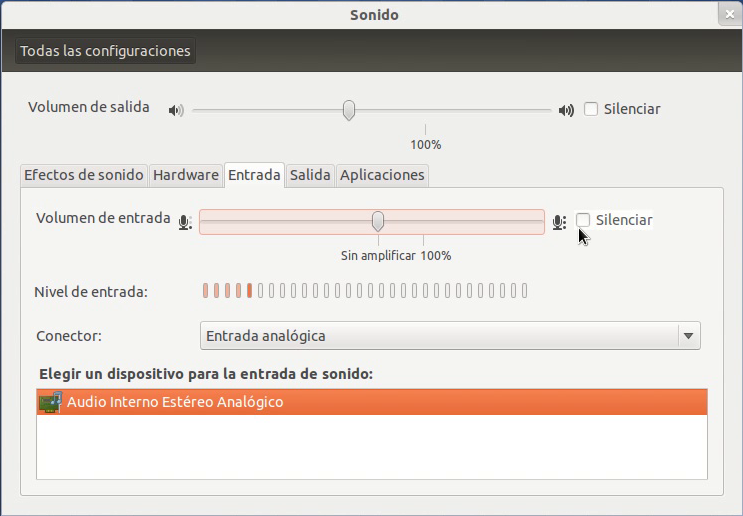
\includegraphics[scale=0.6]{gnome/entSon.png} 
\end{center}
\item{\bf Salida}\\
De la misma manera que en entrada, puedes elegir el conector de la salida de audio.\\
Si el conector de salida es esteréo, tendra la opción de balanceo de sonido.(balance)
\begin{center}
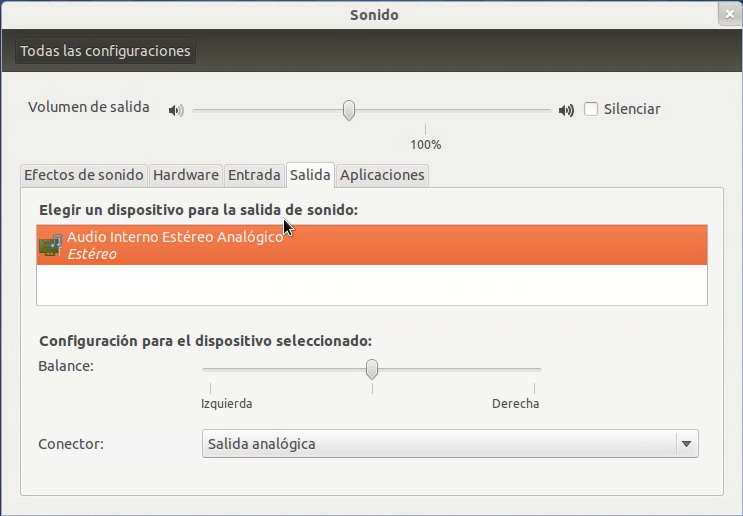
\includegraphics[scale=0.6]{gnome/salson.png} 
\end{center}
\item{\bf Aplicaciones}\\
Independientemente de las opciones de sonido de los conectores(entrada/salida) de sonido, varias aplicaciones tienen sus opciones de emisión de y captura de sonido.\\
Si una aplicación que esta en ejecución, tiene la opción independiente de regular su volumen se mostrara en esta opción de sonido.
\begin{center}
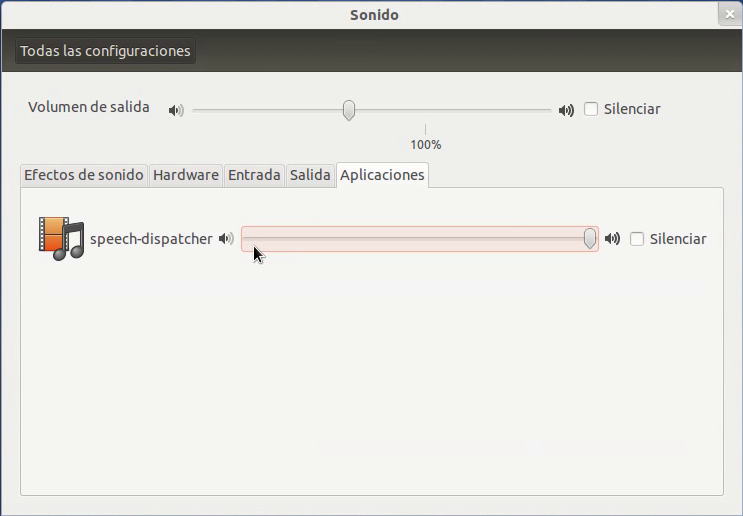
\includegraphics[scale=0.6]{gnome/aplison.png} 
\end{center}
\end{itemize}
\subsection{Soportes extraíbles}
Se pueden utilizar una gran variedad de unidades y soportes extraíbles, incluidos dispositivos de almacenamiento, cámaras y escáneres, entre otros. La configuración de muchos de estos dispositivos se establece automáticamente durante la instalación. Para cambiar la configuración de una unidad o de otro dispositivo extraíble.
\begin{center}
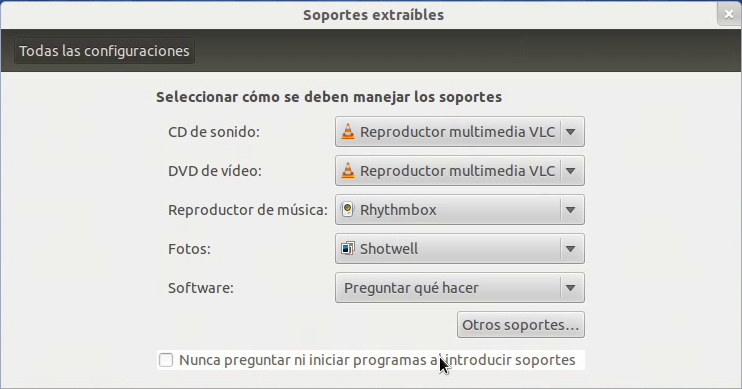
\includegraphics[scale=0.8]{gnome/extraib.png}
\end{center}
Algunos de los ajustes de configuración posibles incluyen:
\begin{itemize}
\item Qué ocurre cuando se introduce un CD vacío en la unidad de CD
\item Qué ocurre cuando se introduce un CD de audio en la unidad
\item Si las imágenes se importan automáticamente desde una cámara digital cuando se conecta al equipo
\item Si los dispositivos de almacenamiento extraíbles se montan cuando se conectan al equipo
\item Si los PDA se sincronizan automáticamente cuando se conectan al equipo
\begin{multicols}{2}
Presionando en otros soportes puede usted asignar que hacer con los dispositivos de almacenamiento

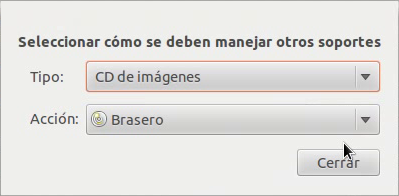
\includegraphics[scale=0.5]{gnome/otrs.png} 
\end{multicols}
\end{itemize}
En general, no es preciso cambiar los ajustes que ya estén configurados a menos que quiera modificar el comportamiento del equipo cuando se conecte un dispositivo o en caso de que quiera conectar un dispositivo nuevo que no esté configurado todavía. Si se conecta un dispositivo por primera vez y se comporta de modo inesperado, compruebe los valores de Unidades y soportes extraíbles.

\section{Sistema}
\subsection{Acceso universal}
Acceso universal es una tecnología de asistencia para dar soporte a usuarios con diversas deficiencias y necesidades especiales y para interactuar con dispositivos de asistencia comunes como:
\begin{itemize}
\item Deficiencias auditivas.
\item Deficiencias motoras.
\end{itemize} 
Se puede acceder a muchas características de accesibilidad desde el menú en la barra superior del escritorio.
Algunos de los ajustes de configuración disponibles incluyen:
\begin{itemize}
\item Ceguera
\item Visión deficiente
\item Movimiento del ratón
\item Pulsar y soltar
\item Uso del teclado
\item El tiempo que se debe mantener pulsada una tecla para que se identifique como
una entrada válida
\item Si el teclado se puede usar como ratón
\item Si las combinaciones en las que se emplean Alt, ControlMayús se pueden duplicar con “teclas persistentes”
\end{itemize}
\begin{itemize}
\item DEFICIENCIAS VISUALES.
\begin{itemize}
\item Ceguera
\begin{description}
\item[lector de pantalla] GNOME proporciona el lector de pantalla Orca para leer la interfaz de usuario. Orca también puede mostrar la interfaz de usuario en dispositivos Braille.\\
Dependiendo de cómo haya instalado GNOME, puede no tener Orca instalado Instale Orca y después, para obtener más información, lea la Ayuda de Orca.
\end{description}
\item Visión deficiente
   \begin{description}
  	\item[Ajustar el contraste] Puede ajustar el contraste de las ventanas y los botones 		para que se vean más fácilmente. Esto no es lo mismo que cambiar el brillo de 				toda la pantalla; solo cambiarán algunas partes de la interfaz de usuario.\\
seleccione el Contraste que mejor se ajuste a sus necesidades. Bajo hará las cosas menos vívidas, por ejemplo.\\
Puede cambiar rápidamente el contraste pulsando en el icono de acceso universal en la barra superior y seleccionando Contraste alto.
  	\item[Cambiar el tamaño del texto en la pantalla] Si tiene dificultades para leer el texto en su pantalla, puede cambiar el tamaño de la tipografía.\\
Seleccione el Tamaño del texto que sea suficientemente grande para usted. Se ajustará inmediatamente.\\
Puede ajustar rápidamente el tamaño del texto pulsando en el icono de accesibilidad en la parte superior de la barra y seleccionando Texto grande.
	\item[Hacer que parpadee el cursor del teclado ] Si tiene dificultades para ver el cursor del teclado en un campo de texto puede hacer que parpadee siendo más fácil ubicarlo.\\
Seleccione Parpadeo del cursor en los campos de texto.\\
Use el deslizador Velocidad para ajustar la rapidez del parpadeo del cursor.
	\item[Localizar rápidamente el puntero] Si tiene problema para ver donde esta el puntero del ratón en su pantalla, podrá localizarlo simplemente pulsando la tecla Ctrl. Al activar esta opción, cuando pulse Ctrl se visualizará una animación que aparecerá brevemente en la posición del puntero.\\
Abra Ratón y touchpad y seleccione la pestaña Mouse.\\
Seleccione Mostrar la posición del puntero al pulsar la tecla Ctrl.\\
Ahora sus teclas Ctrl localizarán el cursor cuando las pulse.
	\item[Magnificar el área de la pantalla] Magnificar la pantalla no es simplemente aumentar el tamaño del texto. Esta característica es como tener una lupa que puede mover aumentando partes de la pantalla.\\
Seleccione la pestaña Visión.\\
Active la Ampliación.
\end{description}
\end{itemize}
\item DEFICIENCIAS AUDITIVAS.
	\begin{description}
		\item de pantalla para sonidos de alerta] Su equipo reproducirá un sencillo sonido de alerta para ciertos tipos de mensajes y eventos. Si tiene dificultades para oír esos sonidos, puede hacer que se ilumine la ventana actual o la pantalla completa cada vez que se reproduzca un sonido de alerta.\\
También puede resultar útil si se encuentra en un entorno en el que necesita que su equipo esté en silencio, como en una biblioteca. Consulte y Elija o desactive el sonido de alerta para saber como silenciar el sonido de alerta y activar las alertas visuales.\\
Seleccione la pestaña Audición.\\
Active las Alertas visuales. Seleccione si quiere que destelle la pantalla entera o solo la ventana actual.\\
Puede activar y desactivar rápidamente las alertas visuales pulsando en el icono de accesibilidad en la barra superior y seleccionando Alertas visuales.
	\end{description}
\item DEFICIENCIAS MOTORAS.
	\begin{itemize}
		\item {\large \bf Movimiento del ratón}
			\begin{description}
				\item[Ajustar la velocidad del ratón y del touchpad] Si el puntero se mueve demasiado deprisa o despacio cuando mueve el ratón o usa el touchpad, puede ajustar la sensibilidad del puntero y la aceleración para estos dispositivos.\\
Abra Ratón y touchpad.\\
Ajuste los deslizadores de Aceleración y Sensibilidad hasta que el movimiento del puntero le sea cómodo.\\

La sensibilidad es la velocidad inicial del puntero al mover su ratón.\\
Cuanto más mueva el ratón, más rápidamente se mueve el puntero con relación a su movimiento. Esto le ayuda a mover el puntero por la pantalla sin levantar la mano, mientras que le permite apuntar y pulsar de manera precisa. La aceleración controla este comportamiento.\\

Puede ajustar la sensibilidad y la aceleración de forma diferente para el ratón y el touchpad. A veces la configuración más agradable para un tipo de dispositivo no es la más cómoda para el otro. Solo tiene que configurar las barras de desplazamiento tanto en la pestaña del Ratón como en la del Touchpad.
				\item[Pulsar y mover el puntero del ratón usando el teclado numérico] Si tiene dificultades al usar un ratón u otro dispositivo señalador, puede controlar el puntero del ratón usando el teclado numérico de su teclado. Esta característica se llama teclas de ratón.\\
Seleccione la pestaña Apuntar y pulsar.\\
Active las Teclas del ratón.\\

Compruebe que la tecla Bloq-Num está desactivada. Ahora podrá mover el puntero del ratón usando el teclado numérico.\\
Puede activar y desactivar las teclas del ratón pulsando en el icono de accesibilidad en la barra superior y seleccionando Teclas del ratón.\\

El teclado numérico es un conjunto de botones numéricos de su teclado, normalmente dispuestos en una matriz cuadrada. Si su teclado no tiene teclado numérico (por ejemplo, el teclado de un portátil), puede que tenga que mantener pulsada la tecla Función (Fn) y usar otras teclas de su teclado como un teclado numérico. Si usa esta característica a menudo en un portátil, puede comprar teclados numéricos USB externos.\\
Cada número del teclado numérico se corresponde con una dirección. Por ejemplo, al pulsar la tecla 8 se moverá el puntero hacia arriba y al pulsar 2 se moverá hacia abajo. Al pulsar la tecla 5 se hará una pulsación con el ratón y al pulsarla dos veces rápidamente se hará una doble pulsación.\\
La mayoría de los teclados tiene una tecla especial que permite hacer una pulsación derecha; generalmente está cerca de la barra espaciadora. Sin embargo, tenga en cuenta que esta tecla responde donde está el foco del teclado, no donde está el puntero del ratón. Consulte la Simular una pulsación derecha del ratón para obtener más información sobre cómo hacer una pulsación derecha manteniendo pulsada la tecla 5 o con el botón izquierdo del ratón.\\
Si quiere usar el teclado numérico para teclear números cuando está activada la opción de teclas del ratón, active Bloq-Num. El ratón no se pueden controlar con el teclado numérico mientras esté activado Bloq-Num.
Las teclas numéricas normales, situadas en una fila en la parte superior del teclado, no controlan el puntero del ratón. Solo pueden hacerlo las teclas del teclado numérico.
			\end{description}
		\item {\large \bf Pulsar y soltar}
			\begin{description}
				\item[Ajustar el umbral de arrastre del ratón] Cuando se pulsa sobre algo, no es raro que su mano se mueva un poco durante el tiempo que pasa entre que pulsa el botón y lo suelta. Por esa razón, el proceso de arrastrar solo empieza si se mueve el puntero pasado un cierto umbral, para que no empiece a arrastrar accidentalmente cada vez que pulse sobre algo.\\

Abra Ratón y touchpad y seleccione la pestaña Mouse.\\
En Arrastrar y soltar, ajuste el deslizador del Umbral a un valor que le resulte cómodo. Pruebe a mover la ventana de opciones arrastrando la barra de título para probar el valor actual.\\
Este ajuste afectará tanto a su ratón como a su touchpad, así como a cualquier otro dispositivo apuntador.
				\item[Ajustar la velocidad de la doble pulsación] La doble pulsación solo sucede cuando pulsa el botón del ratón dos veces lo bastante rápido. Si se tarda mucho en pulsar la segunda vez, obtendrá dos pulsaciones separadas, no una doble pulsación. Si tiene dificultados en pulsar el ratón tan deprisa debería incrementar el tiempo de espera.\\

Abra Ratón y touchpad y seleccione la pestaña Mouse.\\
Bajo Tiempo de espera de la pulsación doble, ajuste el deslizador Tiempo de espera a un valor que considere confortable. Use la cara sonriente junto al deslizador para probar su configuración. Una pulsación simple lo hará sonreír. Una pulsación doble lo hará sonreír de oreja a oreja.\\
Si su ratón hace una doble pulsación cuando usted quiere hacer una sola pulsación, aunque haya incrementado el tiempo de espera de la pulsación doble, es posible que esté defectuoso. Pruebe a conectar otro ratón en su equipo y compruebe si funciona correctamente. O también, conecte su ratón en otro equipo distinto y compruebe si el problema persiste.\\
Este ajuste afectará tanto a su ratón como a su touchpad, así como a cualquier otro dispositivo apuntador.
				\item[Simular una pulsación al posicionar el puntero] Puede pulsar o arrastrar simplemente posando el puntero de su ratón sobre un control o un objeto en la pantalla. Es útil si tiene dificultades para mover el ratón y pulsar a la vez. Esta característica se llama pulsación al enfocar o pulsación al posarse.\\
Cuando la pulsación al enfocar está activada puede mover el puntero de su ratón sobre un control, dejar el ratón y esperar un poco hasta que el botón se pulse automáticamente.\\

Seleccione la pestaña Apuntar y pulsar.\\
Active la Pulsación al posarse.\\

Se abrirá la ventana Pulsación al pasar por encima, que siempre estará encima del resto de ventanas. Puede usarla para elegir el tipo de pulsación que deberá aplicarse cuando coloque el ratón sobre un botón. Por ejemplo, si selecciona Pulsación secundaria, el ratón simulará una pulsación con el botón derecho cuando coloque el puntero sobre un botón durante unos pocos segundos.\\
Al pasar el puntero del ratón sobre un botón y no moverse, poco a poco cambiará de color. Una vez totalmente cambiado de color, el botón se pulsará.\\
Ajuste la opción Retardo para controlar cuánto tiempo debe mantener el puntero del ratón para realizar la pulsación.\\
No tiene por qué mantener el ratón perfectamente quieto al realizar una pulsación al pasar por encima. El puntero se puede mover un poco y aún así se hará la pulsación pasado un tiempo. En cambio, no se producirá la pulsación si lo mueve demasiado.\\
Ajuste la opción del Umbral de movimiento para cambiar cuánto se puede mover el puntero y que aún así se siga considerando una pulsación de posicionamiento.
				\item[Simular una pulsación derecha del ratón] Puede hacer que, en lugar de pulsar el botón derecho del ratón, baste con mantener pulsado el botón izquierdo del ratón durante un tiempo para realizar la misma acción. Es útil si tiene dificultades para mover los dedos de una mano de forma individual o si su dispositivo apuntador tiene un solo botón.\\

Seleccione la pestaña Apuntar y pulsar.\\
Active Pulsación secundaria simulada.\\

Puede cambiar la duración de la pulsación del botón izquierdo del ratón antes de que se considere una pulsación con el botón derecho. En la pestaña Apuntar y pulsar, cambie el Retardo de aceptación bajo Pulsación secundaria simulada.\\
Para pulsar con el botón derecho del ratón usando una pulsación secundaria simulada, mantenga pulsado el botón izquierdo del ratón donde normalmente pulsaría con el botón derecho, después suéltelo. Sólo pulsará con el botón derecho una vez que libere el botón del ratón. Si usa las Teclas del ratón esto también le permitirá pulsar con el botón derecho del ratón manteniendo pulsada la tecla 5 de su teclado numérico.\\

En la vista general de Actividades siempre puede realizar una pulsación larga para ejecutar una pulsación con el botón derecho, incluso si esta característica está desactivada. La pulsación larga funciona de forma ligeramente diferente en la vista general: no tiene que liberar el botón para realizar la pulsación con el botón derecho.
			\end{description}
		\item {\large \bf Uso del teclado}
			\begin{description}
				\item[Activar el rechazo de teclas] Active el rechazo de teclas para ignorar las pulsaciones de teclas repetidas rápidamente. Por ejemplo, si tiene temblores de manos que pueden hacer que pulse teclas varias veces cuando solo quiere pulsarlas una vez, debería activar el rechazo de teclas.\\
Pulse en su nombre en la barra superior y seleccione Configuración del sistema.
Seleccione la pestaña Teclear.\\
Active el Rechazo de teclas.\\

Activar y desactivar rápidamente el rechazo de teclas.\\
Puede activar rápidamente el rechazo de teclas, pulsando en el icono de accesibilidad en la barra superior y seleccionando Rechazo de teclas.\\

Use el deslizador Retardo de aceptación para cambiar el tiempo que debe esperar el rechazo de teclas antes de registrar otra tecla pulsada después de la pulsada en primer lugar. Seleccione Pitar al rechazar una tecla si quiere que el equipo emita un sonido cada vez que ignora una tecla porque la pulsación ha sucedido demasiado pronto después de la pulsación de la tecla anterior.
				\item[Activar las teclas lentas] Active las teclas lentas si quiere que haya un retardo entre la pulsación de una tecla y la visualización de esa letra en la pantalla. Esto significa que tendrá que mantener pulsada un poco cada tecla que desea teclear antes de que aparezca. Use las teclas lentas si pulsa accidentalmente varias teclas a la vez cuando teclea, o si le resulta difícil pulsar la tecla adecuada en el teclado la primera vez.\\
				
Seleccione la pestaña Teclear.\\
Active las Teclas lentas.\\

Activar y desactivar rápidamente las teclas lentas.\\
Seleccione Activar las características de accesibilidad desde el teclado para activar y desactivar las teclas lentas desde el teclado. Cuando esta opción está seleccionada puede pulsar y mantener pulsada la tecla Mayúsculas durante ocho segundos para activar o desactivar las teclas lentas.\\
También puede activar las teclas lentas pulsando el icono de acceso universal en la barra superior y cambie Teclas lentas.

Use el deslizador Retraso de aceptación para controlar cuanto tiempo debe mantener pulsada la tecla para que se registre.\\
Puede hacer que su equipo emita un sonido al pulsar una tecla, cuando se acepta una tecla o al rechazar una tecla porque no la mantuvo pulsada suficiente tiempo.
				\item[Activar las teclas persistentes] Las teclas persistentes le permiten pulsar combinaciones de teclas pulsándolas tecla a tecla, en lugar de tener que mantener pulsadas todas las teclas a la vez. Por ejemplo, la combinación Alt+Tab sirve para pasar de una ventana a otra. Sin las teclas persistentes activadas tendría que mantener pulsadas ambas teclas al mismo tiempo; con las teclas persistentes, puede pulsar la tecla Alt, soltarla y luego pulsar Tab para obtener el mismo resultado.\\
Puede querer activar las teclas persistentes si encuentra dificultad para mantener pulsadas varias teclas a la vez.\\

Seleccione la pestaña Teclear.\\
Active las Teclas persistentes.\\

Activar y desactivar rápidamente las teclas lentas
Seleccione Activar las características de accesibilidad desde el teclado para activar y desactivar las teclas persistentes desde el teclado. Cuando esta opción está seleccionada puede pulsar la tecla Mayúsculas cinco veces seguidas para activar o desactivar las teclas lentas.\\
También puede activar y desactivar las teclas lentas pulsando el icono de acceso universal en la barra superior y cambiando las Teclas lentas.\\

Si pulsa dos teclas a la vez, puede hacer que las teclas persistentes se desactiven temporalmente para introducir un atajo de teclado de la forma estándar.\\
Por ejemplo, si activa las teclas persistentes pero pulsa Alt y Tab simultáneamente, las teclas persistentes no esperaran a que pulse otra tecla si tenia esa opción activada. En cambio, si podría esperar si solo se pulsa una tecla. Esto es útil si puede pulsar algunos atajos de teclado simultáneamente (por ejemplo, con teclas que estén juntas), pero no otras.\\
Seleccione Desactivar si se pulsan dos teclas a la vez para activar esto.\\

Puede hacer que su equipo emita un “pitido” cuando empiece a teclear un atajo de teclado con las teclas persistentes activadas. Esto es útil si quiere que las teclas persistentes esperen que se teclee un atajo de teclado, de manera que la siguiente pulsación se interpretará como parte de un atajo. Seleccione Pitar cuando se presione una tecla modificadora para activar esto.
				\item[Desactivar la repetición de tecla] De manera predeterminada, si mantiene pulsada una tecla en el teclado, se repetirá su letra o símbolo hasta que suelte la tecla. Si tiene dificultades para retirar su dedo lo bastante rápido, puede desactivar esta característica o cambiar el tiempo que tardan los caracteres en empezar a repetirse.\\
				
Abra Teclado y seleccione la pestaña Escritura.\\
Desactive la opción Las pulsaciones de teclas se repiten cuando la tecla se mantiene pulsada para desactivar completamente la repetición de teclas. Alternativamente, ajuste el deslizador Retardo para controlar cuánto tiene que mantener pulsada una tecla hasta que se empiece a repetir y ajuste la Velocidad para controlar cómo de rápido se repiten las pulsaciones de tecla
				\item[Usar un teclado en pantalla] Si no tiene un teclado conectado a su equipo o si prefiere no usarlo, puede activar el teclado en pantalla para escribir texto.\\
				
Seleccione la pestaña Teclear.\\
Active el Teclado en pantalla.\\

Pulse el botón 123 para escribir números y símbolos. Hay más símbolos disponibles si pulsa los botones $\{\#$*. Para volver al teclado alfabético, pulse los botón Abc.\\
Si el teclado en pantalla se interpone, pulse el botón teclado junto al botón de la bandeja para ocultarlo. Para mostrar el teclado, abra la bandeja de mensajes y pulse el elemento del teclado en la bandeja. 
			\end{description}
	\end{itemize}
\end{itemize}



%---------------------------------  (Control, Alt, Supertecla o la tecla de Windows)
	\subsection{Fecha y Hora}
	Si la fecha y hora mostradas en la barra superior son incorrectas, o tienen el formato incorrecto, puede cambiarlas:\\
\begin{itemize}
\item {\large \bf Cambiar la fecha y la hora}\\
Selecciones fecha y hora.
Puede que necesite Desbloquear y escribir la contraseña de administrador.\\
Ajuste la fecha y hora pulsando en las flechas para elegir el año, día, hora y minuto. Puede elegir el mes de una lista desplegable.\\
Si quiere, puede tener su reloj actualizado automáticamente activando la Hora de red.\\
Cuando hora de red está encendido, el equipo sincronizará periódicamente su reloj con un reloj muy preciso en Internet, de manera que no tendrá que hacerlo manualmente. Esto solo funcionará si está conectado a Internet.\\
También puede cambiar el formato de hora, activando o desactivando el formato 24 horas.
\item {\large \bf Cambiar su zona horaria}\\
Pulse en su ubicación actual en el mapa, a continuación, seleccione su ciudad actual en la lista desplegable.\\
La hora que muestra el reloj no se actualizará automáticamente cuando seleccione una ubicación diferente. La hora en la ventana se actualizará la siguiente vez que acceda a la ventana Configuración de fecha y hora. Puede querer establecer la hora manualmente.
		\begin{center}
			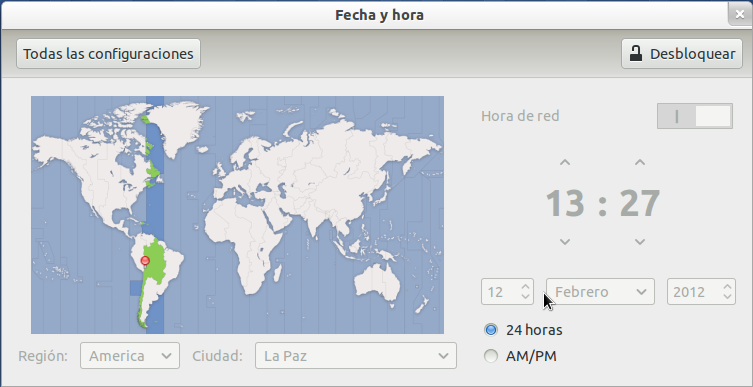
\includegraphics[scale=0.65]{gnome/fechaHora.png} 
		\end{center}
\end{itemize}
\chapter{Acceso a carpetas}
\begin{center}
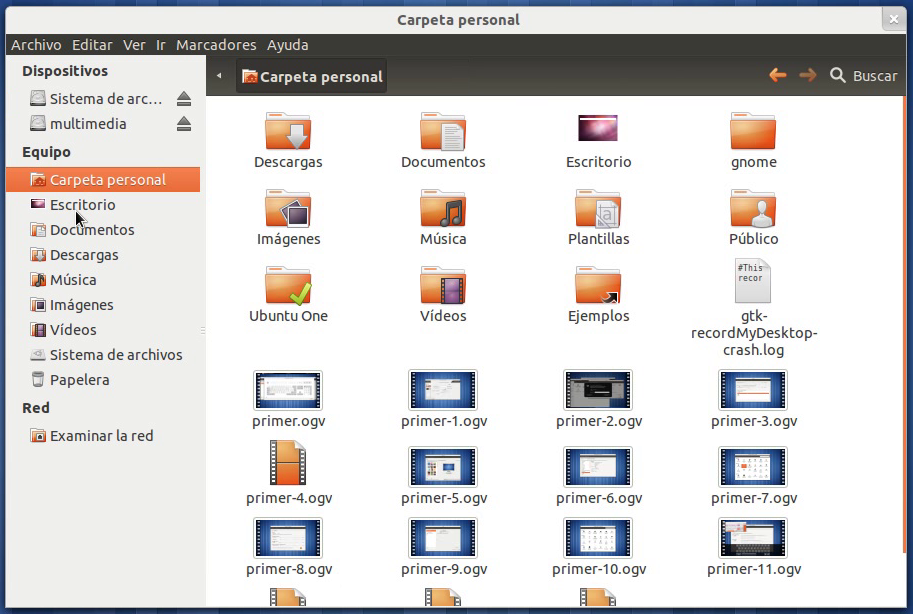
\includegraphics[scale=0.6]{gnome/carpetass.png}
\end{center}
Existen varios gestores de archivos en linux.
Nautilus, es el gestor gráfico de archivos de Gnome, muy fácil de usar.
\begin{itemize}
\item Tiene barra lateral, que se ve muy bien y permite organizar tus “lugares” de forma más sencilla y fácil para navegar por el árbol de directorios.
\item Incorpora una barra de herramientas novedosa e información inteligente de estado.
\item Puede conectarse a un servidor de archivos.
\end{itemize}
A continuación veremos las diferentes tareas de nautilus:
\section{Tareas comunes}
\subsubsection{Examinar archivos y carpetas}
Use la aplicación Archivos para navegar y organizar los archivos en su equipo. También puede usarlo para gestionar archivos en dispositivos de almacenamiento (como discos externos), en servidores de archivos y en recursos compartidos de la red.\\
Para abrir el gestor de archivos, entras en actividades. escribes nautilus y enter si te sale el gestor de archivos.\\
Para pulse acceder a cualquier carpeta pulsa dos veces sobre una carpeta para ver su contenido, o sobre un archivo para abrirlo con la aplicación predeterminada para ese archivo. También puede pulsar con el botón derecho sobre una carpeta para abrirla en una pestaña o una ventana nueva.\\ 
En la vista de lista, también puede pulsar en el extensor situado junto a la carpeta para mostrar su contenido en forma de árbol.\\
Al examinar los archivos en una carpeta puede previsualizar rápidamente cada archivo rápidamente pulsando la barra espaciadora para asegurarse de que tiene el archivo correcto antes de abrirlo, copiarlo o eliminarlo.\\
La barra de rutas situada encima de la lista de archivos y carpetas muestra qué carpeta esta visualizando, incluyendo sus carpetas padre hasta su carpeta personal. Pulse en una carpeta padre de la barra de rutas para moverse a esa carpeta. Pulse con el botón derecho sobre cualquier carpeta de la barra de rutas para abrirla en una pestaña o ventana nueva, copiarla, moverla o acceder a sus propiedades.\\
Si quieres saltar rápidamente a un archivo en la carpeta que está viendo, empiece a escribir su nombre. Aparecerá una caja de búsqueda en la parte inferior de la ventana y se resaltará el primer archivo que coincida con su búsqueda. Pulse la flecha abajo , Ctrl+G o desplácese con el ratón para saltar al siguiente archivo que coincida con su búsqueda.\\
Puede acceder rápidamente a lugares comunes desde la barra lateral. Si no ve la barra lateral, pulse en Ver $>$ Barra lateral $>$ Mostrar barra lateral. Puede añadir marcadores a carpetas que use con frecuencia y aparecerán en la barra lateral. Use el menú Marcadores para hacer esto, o simplemente arrastre una carpeta a la barra lateral.\\
Si mueve frecuentemente archivos entre carpetas anidadas, puede encontrar útil mostrar un árbol en la barra lateral. Pulse Ver $>$ Barra lateral $>$ Árbol, para activar el árbol de la barra lateral. Pulse el expansor junto a la carpeta para mostrar sus carpetas hijas en el árbol, o pulse en una carpeta para abrirla en la ventana.
\subsubsection{Buscar archivos}
Puede buscar archivos según su nombre o su tipo de archivo directamente desde el gestor de archivos. También puede guardar búsquedas frecuentes, que aparecerán como carpetas especiales dentro de su carpeta personal.\\

{\large \bf Buscar}
\begin{enumerate}
\item Abra la aplicación Archivos desde la vista de Actividades.
\item Si sabe que los archivos que quiere buscar están en una carpeta determinada, vaya a esa carpeta.
\item Pulse Buscar en la barra de herramientas, o pulse Ctrl+F.
\item Teclee una o varias palabras que sepa que aparecen en el nombre del archivo y pulse Intro. Por ejemplo, si todas sus facturas contienen en su nombre la palabra Factura, teclee factura. Pulse Intro No hace falta tener en cuenta las mayúsculas y minúsculas.
\item Puede acotar los resultados por ubicación y tipo de archivo. Pulse el botón + para establecer más criterios de búsqueda.
\begin{itemize}
\item Para acotar los resultados de la búsqueda, seleccione Ubicación de la lista desplegaba para añadir una ubicación padre.
\item Para acotar los resultados de la búsqueda en función del tipo de archivo, seleccione Tipo de archivo de la lista desplegable.
Pulse el botón - junto a cualquier opción de búsqueda para quitar esa opción y aumentar los resultados de búsqueda.
\end{itemize}
\item Puede abrir, copiar, eliminar o trabajar con sus archivos desde los resultados de búsqueda, igual como si estuviera en cualquier carpeta en el gestor de archivos.
\item Pulse de nuevo Buscar en la barra de herramientas para salir de la búsqueda y volver a la carpeta.
\end{enumerate}
Si lleva a cabo ciertas búsquedas muy a menudo, puede guardarlas para acceder a ellas rápidamente.\\

{\large \bf Guardar una búsqueda}
\begin{enumerate}
\item Iniciar una búsqueda como la de arriba.
\item Cuando esté satisfecho con sus parámetros de búsqueda, pulse Archivo $>$ Guardar búsqueda como.
\item Asigne un nombre a la búsqueda y pulse Guardar. Si lo desea, seleccione una carpeta distinta en la que guardarla. Cuando visualice esa carpeta, verá sus búsquedas guardadas como un icono de carpeta color naranja con una lupa.
\end{enumerate}
Para eliminar el archivo buscado cuando haya terminado con él, simplemente elimínelo de la búsqueda igual que haría con cualquier otro archivo. Cuando elimina una búsqueda guardada, no elimina los archivos que coincidieron con la búsqueda.
\subsubsection{Copiar o mover archivos y carpetas}
Es posible copiar o mover un archivo o carpeta en una nueva ubicación arrastrando y soltando con el ratón, usando los comandos de copiar y pegar, o mediante combinaciones de teclas.\\

Por ejemplo, es posible que quiera copiar una presentación en una tarjeta de memoria para trabajar con ella. O bien, podría hacer una copia de seguridad de un documento antes de realizar cambios en el mismo (y luego utilizar la copia antigua no le gustan los cambios).\\
Estas instrucciones se aplican tanto a los archivos como a las carpetas. Copia y mueve archivos y carpetas de la misma forma.\\

{\bf Copiar y pegar archivos}\\
\begin{enumerate}
\item Seleccione el archivo que quiera copiar, pulsándolo una sola vez.
\item Pulse Editar $>$ Copiar, o Ctrl+C.
\item Vaya a otra carpeta donde quiera poner la copia del archivo.
\item Pulse Editar $>$ Pegar para finalizar la copia del archivo, o pulse Ctrl+V. Ahora habrá una copia del archivo en la carpeta original y en la otra carpeta.
\end{enumerate}

{\bf Cortar y pegar archivos para moverlos}\\
\begin{enumerate}
\item Seleccione el archivo que quiere mover pulsándolo una sola vez.
\item Pulse Editar $>$ Cortar, o Ctrl+X.
\item Vaya a otra carpeta donde quiera mover el archivo.
\item Pulse Editar $>$ Pegar para finalizar el movimiento del elemento o pulse Ctrl+V. El archivo se tomará de su carpeta original y se moverá a la otra carpeta.
\end{enumerate}

{\bf Arrastrar archivos para copiarlos o moverlos}
\begin{enumerate}
\item Abra el gestor de archivos y vaya a la carpeta que contenga el elemento que quiere copiar.
\item Pulse Archivo $>$ Ventana nueva (o pulse Ctrl+N) para abrir una segunda ventana. En la ventana nueva, navegue hasta la carpeta donde quiere copiar o mover el elemento.
\item Pulse y arrastre el elemento de una ventana a la otra. Esto lo moverá si el destino está en el mismo dispositivo, o lo copiará si el destino está en un dispositivo diferente.
\item Por ejemplo, si arrastra un archivo de una memoria USB a su carpeta personal éste se copiará porque lo está arrastrando desde un dispositivo a otro.
\item Para forzar a que se copie el archivo manteniendo pulsada la tecla Ctrl mientras arrastra el archivo, o forzar mover el archivo manteniendo pulsada la tecla Mayús. mientras arrastra el archivo.
\end{enumerate}
Puede pulsar F3 en el gestor de carpetas para obtener una nuevo navegador de carpetas donde podrás realizar todas las mismas operaciones.\\

No puede copiar o mover un archivo en una carpeta de solo lectura. Algunas carpetas son de solo lectura para impedir que pueda hacer cambios en su contenido. Puede hacer que deje de ser de solo lectura
\subsubsection{Eliminar archivos y carpetas}
Si ya no quiere un archivo o carpeta, puede eliminarlo.\\
Cuando elimina un elemento, este se mueve a la carpeta Papelera, donde queda almacenado hasta que vacíe la papelera. Los elementos almacenados en la carpeta Papelera se pueden restaurar a su ubicación original si decide que los necesita, o si se eliminaron accidentalmente.
\begin{enumerate}
\item  Seleccione el elemento que quiere eliminar pulsándolo una sola vez.
\item Pulse Ctrl+Del en su teclado. Alternativamente, arrastre el elemento hasta la Papelera en la barra lateral.
\end{enumerate}
Para eliminar archivos de forma permanente y liberar espacio de disco en su equipo, debe vaciar la papelera. Para vaciar la papelera, pulse con el botón derecho en la Papelera en la barra lateral y seleccione Vaciar la papelera. También puede eliminar elementos individuales de la papelera examinando la misma desde la barra lateral o el menú Ir. Seleccione los archivos que quiere eliminar permanentemente y pulse Ctrl+Supr en su teclado, o pulse con el botón derecho y seleccione \underline{Eliminar permanentemente}.\\

Los archivos eliminados en dispositivos extraíbles puede no ser visibles en otros sistemas operativos, tales como Windows o Mac OS. Los archivos siguen ahí, y estarán disponibles cuando conecte el dispositivo de nuevo en su equipo.\\

{\bf Eliminar permanentemente un archivo}\\
Puede eliminar un archivo permanentemente de forma inmediata, sin tenerlo que enviar primero a la papelera.
\begin{enumerate}
\item Seleccione el elemento que quiere eliminar.
\item Pulse y mantenga pulsada la tecla Mayús, y luego pulse la tecla Supr de su teclado.
\item Como no puede deshacer esta operación, se le preguntará que confirme si quiere eliminar el archivo o carpeta.
\end{enumerate}
Si necesita con frecuencia eliminar archivos sin usar la papelera (por ejemplo, si trabaja a menudo con datos sensibles), puede añadir una opción Eliminar al menú contextual de archivos y carpetas. Pulse Editar $>$ Preferencias y seleccione la pestaña Comportamiento. Seleccione Incluir el comando \underline{Eliminar} que no use la papelera.
\subsubsection{Ordenar archivos y carpetas}
Puede ordenar los archivos de una carpeta de diferentes formas; por ejemplo, por fecha o tamaño. Consulte la Maneras de ordenar archivos a continuación una lista de formas habituales de ordenar archivos.\\
Cuando cambia la manera de ordenar elementos en una carpeta, solo afecta a esa carpeta. El gestor de archivos recordará sus preferencias de ordenación para esa carpeta, pero usará el criterio de ordenación predeterminado en las demás carpetas. Consulte la Preferencias de las vistas del gestor de archivos para obtener más información sobre cómo cambiar el criterio de ordenación predeterminado.\\
La forma en la que ordene los archivos dependerá de la vista de carpeta que esté usando. Puede cambiar la vista actual usando el menú Ver.
\begin{itemize}
\item {\bf Vista de icono}\\
Para ordenar los archivos de forma diferente, pulse con el botón derecho en un lugar vacío de la carpeta y seleccione una opción del menú Organizar los elementos. También puede usar el menú Ver $>$ Organizar los elementos.\\
Por ejemplo, si selecciona Ordenar por nombre en el menú Organizar los elementos, los archivos se ordenarán según sus nombres. Consulte otras opciones en la Maneras de ordenar archivos.\\

Puede ordenar en orden inverso seleccionando Orden inverso en el menú Organizar los elementos.\\
Para controlar totalmente el orden y la posición de los archivos en la carpeta, pulse con el botón derecho en un lugar vacío de la carpeta y seleccione Organizar los elementos $>$ Manualmente. Así podrá reorganizar los archivos arrastrándolos y soltándolos por la carpeta. La ordenación manual solo funciona en la vista de iconos.\\
La opción Disposición compacta del menú Organizar los elementos organiza los archivos de forma que ocupan el menor espacio posible. Es útil si quiere ver un montón de archivos al mismo tiempo en una carpeta.
\item {\bf Vista de lista}\\ Para ordenar los archivos de forma diferente, pulse en una de las cabeceras de las columnas en el gestor de archivos. Por ejemplo, pulse en Tipo para ordenar por tipo de archivo. Pulse de nuevo en la cabecera de la columna para ordenar en orden inverso.\\
En la vista de lista, puede mostrar las columnas con más atributos y ordenar estas columnas. Pulse en Vista $>$ Columnas visibles y seleccione las columnas que desea que sean visible. A continuación, podrá ordenar por esas columnas. Consulte la Preferencias de las columnas en la lista del gestor de archivos para obtener las descripciones de las columnas disponibles.
\item {\bf Vista compacta}\\ Puede ordenar los archivos en la vista compacta de la misma manera que puede ordenar la vista de iconos. La única diferencia es que no se puede colocar manualmente los archivos en cualquier lugar que desee, siempre están organizados en una lista en esta vista.
\item {\bf Maneras de ordenar archivos}\\
\begin{itemize}
\item {\bf Por nombre.-} Ordena alfabéticamente por el nombre del archivo.
\item {\bf Por tamaño.-} Ordena por el tamaño del archivo (cuánto espacio ocupa). Ordena de menor a mayor de manera predeterminada.
\item {\bf Por tipo.-} Ordena alfabéticamente por el tipo de archivo. Los archivos del mismo tipo se agrupan, a continuación, ordenados por nombre.
\item {\bf Por fecha de modificación.-} Ordena por la fecha y hora en las que se modificó un archivo por última vez. Ordena de la más antigua a la más reciente de manera predeterminada.
\end{itemize}
\end{itemize}
\subsubsection{Previsualizar archivos y carpetas}
Puede previsualizar archivos rápidamente sin abrirlos en una aplicación completa. Seleccione un archivo y pulse la barra espaciadora. El archivo se abrirá en una ventana simple de vista previa. Pulse la barra espaciadora de nuevo para cerrar la vista previa.\\
La vista previa soporta la mayoría de formatos de archivo para documentos, imágenes, vídeo y sonido. En la vista previa puede desplazarse por sus documentos o buscar a través de sus vídeos y archivos de sonido.\\
Para ver una vista previa a pantalla completa, pulse el botón f. o pulse la barra espaciadora.
\subsubsection{Renombrar un archivo o una carpeta}
Puede cambiar el nombre de un archivo o de una carpeta.
\begin{enumerate}
\item Pulse con el botón derecho sobre un archivo o carpeta y seleccione Renombrar, o seleccione el archivo y pulse F2.
\item Escriba el nombre nuevo y pulse Intro.
\end{enumerate}
También puede renombrar un archivo desde la ventana de propiedades.\\
Cuando cambia el nombre de un archivo, solo se selecciona la primera parte del nombre de ese archivo, sin la extensión (la parte que va detrás del punto “.”). La extensión normalmente representa el tipo de archivo (p.ej archivo.pdf es un documento PDF), y normalmente no querrá cambiarla. Si necesita cambiar la extensión también, seleccione el nombre completo del archivo y cámbielo.\\

{\bf Problemas comunes}
\begin{itemize}
\item {\bf El nombre ya está en uso}\\
No puede tener dos archivos o carpetas con el mismo nombre en la misma carpeta. Si al cambiar el nombre a un archivo intenta asignarle uno que ya existe en la carpeta donde está trabajando, el gestor de archivos no se lo permitirá. Use un nombre distinto.\\
Los nombres de archivos y carpetas distinguen las mayúsculas y las minúsculas. Por ejemplo, Archivo.txt y archivo.txt son dos nombres diferentes. Esto esta permitido, aunque no siempre es una buena idea.\\
\item {\bf El nombre de archivo demasiado largo}\\
En algunos sistemas de archivos, los nombres de archivos no pueden contener más de 255 caracteres. Use un nombre más corto.
\item {\bf La opción para renombrar está en gris}\\
Si la opción Renombrar aparece en color gris, es que no tiene los permisos necesarios para cambiar el nombre del archivo. Normalmente, si no tiene los permisos adecuados, no debería intentar renombrarlo. Consulte la Establecer los permisos del archivo.
\end{itemize}
\section{Otros temas}
\subsubsection{Abrir archivos con otras aplicaciones}
Cuando se pulsa dos veces sobre un archivo en el gestor de archivos, se abre con la aplicación predeterminada para ese tipo de archivos. Puede abrirlo con una aplicación distinta, buscar aplicaciones en línea, o establecer la aplicación predeterminada para todos los archivos del mismo tipo.\\

Para abrir un archivo con una aplicación distinta de la predeterminada, pulse en el archivo y seleccione la aplicación que desee en la parte superior del menú. Si no ve la aplicación que quiere, pulse en Abrir con otra aplicación. De manera predeterminada, el gestor de archivos solo muestra las aplicaciones que sabe que pueden manejar el archivo. Para buscar todas las aplicaciones en su equipo, pulse en Mostrar otras aplicaciones.\\
Si aun no encuentra la aplicación que quiere, puede buscar más aplicaciones pulsando Buscar aplicaciones en línea. El gestor de archivos buscará en línea paquetes que contengan aplicaciones que manejen archivos de ese tipo.\\

{\bf Cambiar la aplicación predeterminada}\\
Puede cambiar la aplicación predeterminada usada para abrir los archivos de un cierto tipo. Esto le permitirá abrir su aplicación preferida cuando pulse dos veces sobre un archivo para abrirlo. Por ejemplo, puede que quiera que se abra su reproductor de música favorito al pulsar dos veces sobre un archivo MP3.
\begin{enumerate}
\item Seleccione un archivo del tipo cuya aplicación predeterminada desea cambiar. Por ejemplo, para cambiar la aplicación usada para abrir archivos MP3, seleccione un archivo .mp3.
\item Pulse con el botón derecho del ratón y seleccione Propiedades.
\item Seleccione la pestaña Abrir con.
\item Seleccione la aplicación que quiere y pulse Establecer como predeterminada. De manera predeterminada, el gestor de archivos solo muestra aplicaciones que sabe que pueden manejar el archivo. Para buscar entre todas las aplicaciones en su equipo, pulse Mostrar otras aplicaciones.
\end{enumerate}
Si \underline{Otras aplicaciones} contiene una aplicación que desea usar a veces, pero que no quiere convertir en la predeterminada, seleccione esa aplicación y pulse en Añadir. Esto la añadirá a Aplicaciones recomendadas. A partir de entonces podrá usar la aplicación pulsando con el botón derecho sobre el archivo y seleccionándola de la lista.\\

Esto cambiará la aplicación predeterminada no solo para el archivo seleccionado, sino para todos los archivos del mismo tipo.
\subsubsection{Compartir y transferir archivos}
Puede compartir archivos fácilmente con sus contactos o transferirlos a dispositivos externos o a recursos compartidos de la red directamente desde el gestor de archivos.\\
\begin{itemize}
\item Abra la aplicación Archivos desde la vista de Actividades.
\item Seleccione el archivo que quiere transferir.
\item Pulse con el botón derecho del ratón y seleccione Enviar a....
\item Aparecerá la ventana Enviar a. Seleccione a dónde desea enviar el archivo y pulse Enviar.\\ Para obtener más información, consulte la siguiente lista de destinos.
\end{itemize}
Puede enviar varios archivos a la vez. Seleccione varios archivos manteniendo pulsada la tecla Ctrl y pulse con el botón derecho sobre cualquier archivo seleccionado. Podrá comprimir los archivos automáticamente en un archivador tar o zip.\\

{\bf Destinos}\\
\begin{itemize}
\item Para enviar por correo electrónico el archivo, seleccione Correo-e e introduzca la dirección del correo electrónico del destinatario.
\item Para enviar el archivo a un contacto de mensajería instantánea, seleccione Mensaje instantáneo, y seleccione el contacto en la lista desplegable. Para que funcione, es posible que tenga que iniciar su programa de mensajería instantánea.
\item Para grabar el archivo en un CD o DVD, seleccione Creador de CD/DVD. Consulte la Escribir archivo en un CD o DVD para obtener más información.
\item Para transferir el archivo a un dispositivo Bluetooth, seleccione Bluetooth (OBEX Push) y seleccione el archivo al que enviarlo. Sólo verá dispositivos que ya estén emparejados Consulte la Bluetooth para obtener más información.
\item Para copiar el archivo a un dispositivo externo como una memoria flash USB, o subirlo a un servidor al que está conectado, seleccione Soportes extraíbles y comparticiones y a continuación seleccione el dispositivo o servidor en el que quiere copiar el archivo
\end{itemize}
\subsubsection{Encontrar un archivo perdido}
Si ha creado o descargado un archivo, pero no sabe donde esta, siga estas indicaciones.\\
\begin{itemize}
\item Si no recuerda donde guardo el archivo, pero tiene cierta idea de como se llama, puede buscarlo por su nombre. Consulte la Buscar archivos para saber cómo.
\item Si acaba de descargar el archivo, su navegador web podría haberlo guardado automáticamente en una carpeta común. Compruebe las carpetas Escritorio y Descargas en su carpeta personal.
\item Es posible que haya eliminado el archivo accidentalmente. Cuando elimina un archivo, se mueve a la papelera, donde permanecerá hasta que vacíe la papelera manualmente.\\ Consulte la Recuperar un archivo eliminado para saber cómo recuperar un archivo eliminado.
\item Puede que haya cambiado el nombre del archivo de forma que ahora quede oculto. Los archivos que empiezan por . o que acaban en $~$ están ocultos en el gestor de archivos. Pulse Ver $>$ Mostrar los archivos ocultos en el gestor de archivos. Consulte la Ocultar un archivo para obtener más información.
\end{itemize}
\subsubsection{Escribir archivo en un CD o DVD}
Puede poner archivos en un disco vacío usando el Creador de CD/DVD. La opción de crear un CD o un DVD aparecerá en el gestor de archivos tan pronto como introduzca un CD en su grabador de CD/DVD. El gestor de archivos le permite transferir archivos a otros equipos o realizar copias de respaldo poniendo archivos en un disco vacío. Para escribir archivos en un CD o DVD
\begin{enumerate}
\item Coloque un disco vacío dentro de un unidad grabadora de CD/DVD.
\item En la ventana Disco CD/DVD-R vacío que aparece, seleccione Creador de CD/DVD y pulse Aceptar. Se abrirá la ventana de la carpeta del creador de CD/DVD.\\
(También puede pulsar en Disco CD/DVD-R virgen bajo Dispositivos en la barra lateral del gestor de archivos.)
\item En el campo Nombre del disco teclee un nombre para el disco.
\item Arrastre o copie los archivos que quiera a la ventana.
\item Pulse Escribir en el disco.
\item En Seleccione un disco en el que grabar seleccione el disco vacío.\\
(También puede elegir $>$ Archivo de imagen. Esto pondrá los archivos en una imagen de disco, que se guardará en su equipo. Más tarde podrá grabar esa imagen en un disco vacío.)
\item Pulse en Propiedades si desea ajustar la velocidad de grabación, la ubicación de los archivos temporales y otras opciones. Las opciones predeterminadas deberían ser suficientes.
\item Pulse el botón Grabar para comenzar la grabación.\\
Si selecciona Grabar varias copias, se le pedirá que introduzca más discos.
\item Cuando se haya grabado el disco por completo, se expulsará automáticamente. Seleccione Hacer más copias o Cerrar para salir.
\end{enumerate}
{\bf Si el disco no se grabó correctamente}\\
A veces, los discos no se graban correctamente y no podrá ver los archivos que puso en el disco cuando lo introduzca en un equipo.\\
En este caso, pruebe a grabar de nuevo el disco usando una velocidad de grabación más lenta; por ejemplo 12x en lugar de 48x. Grabar a velocidades más lentas es más fiable. También puede seleccionar la velocidad pulsando en el botón Propiedades de la ventana Carpeta del creador de CD/DVD.
\subsubsection{Examinar archivos en un servidor o compartición de red}
Puede conectarse a un servidor o a un recurso compartido para buscar y ver los archivos en el servidor, exactamente como si estuvieran en su máquina local o dispositivo extraíble. Esta es una manera conveniente para descargar o subir archivos, o para compartir archivos con usuarios en su red local.\\
Para examinar archivos en la red abra la aplicación de Archivos desde la vista general de Actividades. Después pulse Navegar por la red en la barra lateral, o seleccione Red en el menú Ir. El gestor de archivos buscará cualquier equipo en su red local que informe que puede servir archivos. Si quiere conectarse a un servidor de Internet, o si no ve el equipo que está buscando, puede conectarse manualmente a un servidor introduciendo su dirección de red o internet.\\

{\bf Conectar con un servidor de archivos}\\
\begin{enumerate}
\item En el gestor de archivos pulse Archivo $>$ Conectar con el servidor.
\item Introduzca la dirección del servidor, seleccione el tipo de servidor y escriba cualquier información adicional cuando se le solicite. Después, pulse en Conectar. Se listan debajo detalles acerca de los tipos de servidores.\\
Para servidores en Internet, generalmente se puede usar el nombre de dominio (ej. ftp.ejemplo.com). Sin embargo, para los equipos de su red de área local, puede que tenga que usar la dirección IP numérica del equipo.
\item Se abrirá una nueva ventana mostrando los archivos en el servidor. Puede examinar los archivos de igual forma que si estuviesen en su mismo equipo.\\

El servidor también se añadirá a la barra lateral para que pueda acceder rápidamente a él en el futuro
\end{enumerate}
{\bf Diferentes tipos de servidores}\\
Puede conectarse a diferentes tipos de servidores. Algunos servidores son públicos, y permiten a cualquiera conectarse. Otros servidores requieren que inicie sesión con su nombre de usuario y contraseña.\\
Puede que no tenga permisos para realizar ciertas acciones sobre los archivos en un servidor. Por ejemplo, en sitios FTP públicos, probablemente no podrá eliminar archivos.\\

{\bf Tipos de servidores}
\begin{itemize}
\item {\bf SSH}\\
Si tiene una cuenta SSH en un servidor, podrá conectarse usando este método. Muchos servidores de alojamiento web proporcionan cuentas SSH a sus miembros para que puedan subir archivos de forma segura. Los servidores SSH siempre requieren que usted inicie una sesión. Si usa una clave de SSH para iniciar sesión, deje el campo de contraseña en blanco.\\
Cuando se usa SSH, todos los datos que envía (incluyendo su contraseña) van cifrados, por lo que otros usuarios de su red no podrán verlos.
\item {\bf FTP (con registro)}\\
FTP es un protocolo muy popular para intercambiar archivos por Internet. Dado que los datos no están cifrados a través de FTP, muchos servidores ahora facilitan el acceso a través de SSH. Algunos servidores, sin embargo, todavía permiten o requieren el uso de FTP para subir o descargar archivos. Los sitios FTP con inicio de sesión generalmente le permitirán eliminar y subir archivos.
\item {\bf FTP público}\\
Los sitios que le permiten descargar archivos a veces proporcionan acceso FTP público o anónimo. Estos servidores no requieren un nombre de usuario y contraseña, y por lo general no le permiten eliminar o subir archivos.\\
Algunos sitios FTP anónimos requieren iniciar sesión con un nombre de usuario y contraseña pública, o con un nombre de usuario público utilizando su dirección de correo electrónico como contraseña. Para estos servidores, utilice el método de FTP (con entrada), y use las credenciales especificadas por el sitio FTP.
\item {\bf Compartición Windows}\\
Los equipos Windows usan un protocolo privativo para compartir archivos a través de una red de área local. Los equipos de una red Windows a veces se agrupan en dominios para organizar y controlar mejor el acceso. Si tiene los permisos adecuados en el equipo remoto, podrá conectarse a un recurso compartido de Windows desde el gestor de archivos.
\item {\bf WebDAV y WebDAV seguro}\\
Basado en el protocolo HTTP usado en la web, a veces se usa WebDAV para compartir archivos en una red local o guardarlos en Internet. Si el servidor al que se esta conectando admite conexiones seguras, debería escoger esta opción. WebDAV seguro usa cifrado SSL fuerte, por lo que nadie podrá ver su contraseña ni sus datos.
\end{itemize}
\subsubsection{Propiedades del archivo}
Puede ver información sobre un archivo o carpeta, pulse con el botón derecho y seleccione Propiedades. También puede seleccionar el archivo y pulsar Alt+Intro.\\

La ventana de propiedades del archivo le muestra información tal como el tipo de archivo, su tamaño y cuándo lo modificó por última vez. Si necesita esta información a menudo, puede mostrarla en las columnas de la vista de lista o en las leyendas de los iconos.\\
La información básica dada en la pestaña Básico se explica a continuación. También están las pestañas Permisos y Abrir con. Para ciertos tipos de archivos, como imágenes y vídeos, habrá una pestaña adicional que proporcione información sobre el tamaño, la duración y el codec.\\

{\bf Propiedades básicas}
\begin{itemize}
\item {\bf Nombre}\\
Puede cambiar el nombre del archivo cambiando este campo. También puede cambiar el nombre de un archivo fuera de la ventana de propiedades. Consulte la Renombrar un archivo o una carpeta.
\item {\bf Tipo}\\
El tipo de un archivo, como documento PDF, texto de OpenDocument o imagen JPEG. El tipo MIME del archivo determina qué aplicaciones pueden abrir el archivo, entre otras cosas.Por ejemplo, no puede abrir una imagen con un reproductor de música. Consulte la Abrir archivos con otras aplicaciones para obtener más información.\\
Entre paréntesis se muestra el tipo MIME del archivo; el tipo MIME es una forma estándar que los equipos usan para referirse al tipo de archivo.
\item {\bf Contenido}\\
Este campo se muestra si está consultando las propiedades de una carpeta. Muestra el número de elementos de la carpeta. Si la carpeta incluye otras carpetas, cada carpeta interna se cuenta como un elemento, aunque contenga a su vez otros elementos. Cada archivo se cuenta como un elemento. Si la carpeta está vacía, el contenido no mostrará nada.
\item {\bf Tamaño}\\
Este campo se muestra si está viendo un archivo (no una carpeta). el tamaño de un archivo le indica cuanto espacio ocupa en el disco. También es un indicador de cuánto tardará en descargar un archivo o en enviarlo por correo-e (cuanto más grande es el archivo, más tarda al enviarse/recibirse).\\
Los tamaños se puede dar en bytes, KBs, MBs o GBs; en los tres últimos casos, el tamaño en bytes aparece entre paréntesis. Técnicamente, 1Kb son 1024 bytes, 1MB son 1024 KB, y así sucesivamente.
\item {\bf Ubicación}\\
La ubicación de cada archivo en su sistema viene dada por su ruta absoluta. Esto es una dirección única del archivo en el equipo, compuesta de una lista de carpetas a las que debe ir para encontrar el archivo. Por ejemplo, si Jaime tiene un archivo Resumen.pdf en su carpeta personal, la ubicación será /home/jaime/Resumen.pdf.
\item {\bf Volumen}\\
El sistema de archivo o el dispositivo en el que está almacenado el archivo. Esto le muestra dónde está almacenado físicamente el archivo, por ejemplo, si está en el disco duro, en un CD o en una carpeta de red o un servidor de archivos. Los discos duros se pueden dividir en varias particiones; la partición se mostrará también debajo del Volumen.
\item {\bf Espacio libre}\\
Esto sólo se muestra para las carpetas. Indica la cantidad total de espacio disponible en el disco en el que se encuentra la carpeta. Es útil para comprobar si el disco duro está lleno.
\item {\bf Accedido}\\
Fecha y hora de la última apertura del archivo.
\item {\bf Modificado}\\
Fecha y hora de la última vez que se cambió y guardó el archivo.
\end{itemize}
\subsubsection{Recuperar un archivo eliminado}
Si ha eliminado un archivo pulsando Ctrl+Supr, pulsando el elemento de menú Mover a la papelera o arrastrando el archivo a la papelera, el archivo debería estar en la papelera.\\

{\bf Restaurar desde la papelera}
\begin{enumerate}
\item Abra la aplicación Archivos desde la vista de Actividades.
\item Pulse Papelera en la barra lateral.
\item Si su archivo eliminado está ahí, pulse con el botón derecho sobre él y seleccione \underline{Restaurar}. Se devolverá a la carpeta de la que se borró
\end{enumerate}
Si eliminó el archivo usando Mayús+Eliminar o desde la línea de comandos, el archivo no se podrá recuperar usando este método porque se habrá eliminado permanentemente.\\
Existen varias herramientas de recuperación disponibles que a veces pueden recuperar archivos que se eliminaron permanentemente. No obstante, normalmente no son muy fáciles de usar. Si eliminó un archivo permanentemente de forma accidental, probablemente sea mejor pedir ayuda en los foros de soporte para ver si es posible recuperarlo.
%%\subsubsection{Preferencias del gestor de archivos}


\chapter{Uso de application launcher}
En este capitulo aprenderemos la forma mas rápida de iniciar aplicaciones\\

Mueva el puntero de su ratón a la esquina de Actividades en la parte superior izquierda de la pantalla para mostrar la Vista de actividades. Aquí es donde puede encontrar todas sus aplicaciones. (También puede abrir la vista pulsando la supertecla o tecla windows.)
Hay distintas maneras de abrir una aplicación una vez que está en la vista de actividades:
\begin{itemize}
\item Comience a escribir las primeras letras de una aplicación; y la búsqueda comenzará al instante. (Si esto no sucede, pulse en la barra de búsqueda en la parte superior derecha de la pantalla y comience a escribir.) Pulse en el icono de la aplicación para iniciarla.
\item Pulse en la cabecera de Aplicaciones en la parte superior de la pantalla para ver una lista de aplicaciones que puede ejecutar. Puede filtrar por tipo, usando las categorías de la derecha, o buscar mediante la barra de búsqueda en la parte superior derecha. Pulse en el icono de la aplicación para iniciarla.
\item Algunas aplicaciones tienen iconos en el tablero, la franja vertical de los iconos en el lado izquierdo de la vista de actividades. Pulse en uno de ellos para iniciar la aplicación correspondiente.\\
Si tiene aplicaciones que usa muy frecuentemente, puede añadirlas al tablero.
\item Puede iniciar una aplicación en un área de trabajo independiente arrastrando el icono de la aplicación desde el tablero (o desde la lista de aplicaciones), y colocándolo en una de las áreas de trabajo en la parte derecha de la pantalla. La aplicación se abrirá en el área de trabajo que elija.
\end{itemize}
Por ejemplo, para lanzar el gestor de archivos, escriba “nautilus” (sin las comillas). El nombre de la aplicación es el comando para lanzar el programa.
\begin{center}
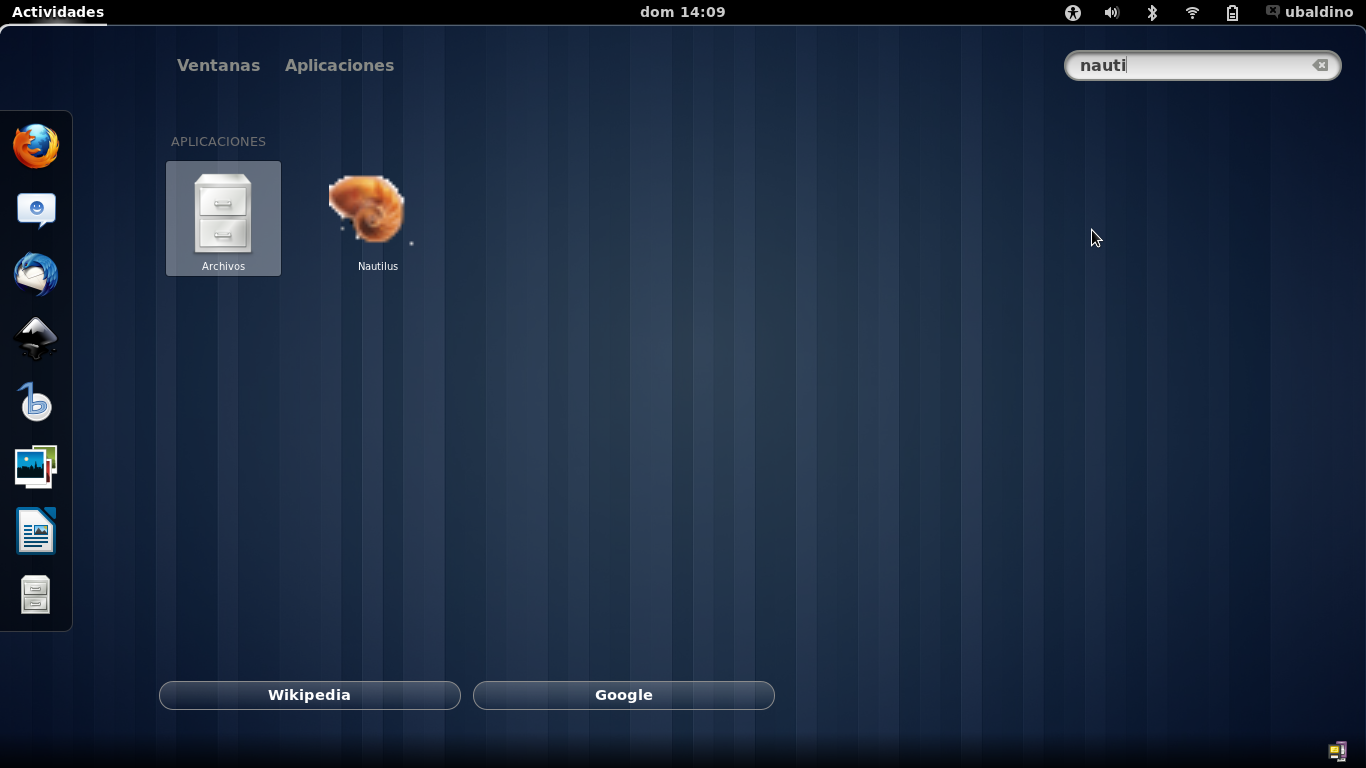
\includegraphics[scale=0.35]{gnome/Pantallazo9.png} 
\end{center}
\end{document}
